\documentclass[12pt,phd,times]{pkmthesis}

\usepackage{amsmath,epsfig,graphicx,setspace,url,float}
\usepackage{pstricks,colortab,pifont}
\usepackage{lscape,multicol,multirow,longtable,subfigure}
\usepackage{cite, bm}   
\usepackage{geometry}
\usepackage{array}
\usepackage{algorithm}
\usepackage{multirow}
\usepackage{tabularx}
\usepackage{graphicx}
\usepackage[small,bf]{caption}              % Added on 26/08/08 (moved before subcaption to avoid option-clash with modern caption pkg)
\usepackage{subcaption}
\usepackage{booktabs}% Due to this hyberref will not work for references (PKM on 07/07/08)
\usepackage[english]{babel}
%\usepackage{slashbox} 
\usepackage{csquotes}  
\usepackage{threeparttable}
%\usepackage{adjustbox}                    % Added on 24/10/08 (Senthil)
\setlength{\textfloatsep}{1cm}              % Spacing b/w  float and text (PKM 01/11/08)
%..........................................................................................................................................
\normalem                                   % Added on 01/07/08 to avoid underline in the references
\setlength{\abovecaptionskip}{8pt}          % Added on 08/07/08
\setlength{\belowcaptionskip}{8pt}          % Added on 08/07/08
%..........................................................................................................................................
\usepackage{hyperref}
\usepackage{extra_functions}
\usepackage{tikz}
\usetikzlibrary{arrows.meta,positioning,fit,shapes.geometric}
%\input{pagesetup_pkm_twoside.tex}           % Modified on 06/07/08, 10/07/08, 15/07/08
%\input{pagesetup_pkm_singleside.tex}       % For Single Sided Document 
\input{pagesetup_pkm_middleside.tex}       % Middle alignment 
\raggedbottom                               % o6/08/08  (Remove Unnecessary space b/w paragraphs)
%******************************************************************************************************************************************

\begin {document}
\setcounter{page}{1} \pagenumbering{roman}  % 03/07/08
\doublespacing                              % or use \baselineskip 12pt (12, 18 and 24)
%*************************************************** FRONT PAGES**********************************************
%\thispagestyle{empty}
%\pdfbookmark{Title}{Title}
%\begin{singlespace}
\begin{center}
\fontsize{15.8pt}{19pt}\selectfont
{\textbf{Event-Driven Traffic Congestion Severity Prediction\\
and Resource Recommendation System \\}}
\vspace*{0.12in}
\emph{\large{A \\
report submitted in fulfillment for the award of the degree of}} \\
\emph{\large{Bachelor of Technology \\}}
\large{in \\}
\large{Information Technology\\}
\large{Bachelor of Technology Project \\}
\large{\textbf{Final Evaluation Report}}

\vspace*{0.12in}
\large{By}\\
\large{\textbf{Aman Kumar (2023IMT-010)}} \\
\large{\textbf{Viswajit Sarak Patil (2023IMT-071)}} \\
\large{\textbf{Sahil Pal (2023IMT-069)}} \\
\vspace*{0.08in}
\large{Under the Supervision of} \\
\large{\textbf{Dr. Saswata Roy}} \\
\large{Department of Information Technology}
\end{center}
\begin{figure}[!h]
\centering
\includegraphics*[width = 2.6cm]{FrontPages/ABV_IIITM_logo.eps}
\end{figure}
\begin{center}
\large{ABV-INDIAN INSTITUTE OF INFORMATION TECHNOLOGY} \\
\large{AND MANAGEMENT GWALIOR}
\vspace*{0.05in}

\large{GWALIOR, INDIA}
\vspace*{0.05in}

\large{August 2026}
\end{center}
\end{singlespace}

%\thispagestyle{empty}
%\clearpage

\thispagestyle{empty}
\pdfbookmark{Title}{Title}
\begin{singlespace}
\begin{center}
\fontsize{15.8pt}{19pt}\selectfont
{\textbf{Event-Driven Traffic Congestion Severity Prediction\\
and Resource Recommendation System \\}}
\vspace*{0.12in}
\emph{\large{A \\
report submitted in fulfillment for the award of the degree of}} \\
\emph{\large{Bachelor of Technology \\}}
\large{in \\}
\large{Information Technology\\}
\large{Bachelor of Technology Project \\}
\large{\textbf{Final Evaluation Report}}

\vspace*{0.12in}
\large{By}\\
\large{\textbf{Aman Kumar (2023IMT-010)}} \\
\large{\textbf{Viswajit Sarak Patil (2023IMT-071)}} \\
\large{\textbf{Sahil Pal (2023IMT-069)}} \\
\vspace*{0.08in}
\large{Under the Supervision of} \\
\large{\textbf{Dr. Saswata Roy}} \\
\large{Department of Information Technology}
\end{center}
\begin{figure}[!h]
\centering
\includegraphics*[width = 2.6cm]{FrontPages/ABV_IIITM_logo.eps}
\end{figure}
\begin{center}
\large{ABV-INDIAN INSTITUTE OF INFORMATION TECHNOLOGY} \\
\large{AND MANAGEMENT GWALIOR}
\vspace*{0.05in}

\large{GWALIOR, INDIA}
\vspace*{0.05in}

\large{August 2026}
\end{center}
\end{singlespace}

\thispagestyle{empty}

\clearpage
\thispagestyle{empty}
\pdfbookmark{Dedication}{Dedication}
%\include{FrontPages/Dedication}
\newpage
\thispagestyle{empty}
\clearpage
\thispagestyle{empty}
\pdfbookmark{Certificate}{Certificate}

\begin{center}
{\Large \bf DECLARATION}
\end{center}
\vspace{0.5cm}
\noindent We hereby certify that the work, which is being presented in this report, entitled \textbf{``Event-Driven Traffic Congestion Severity Prediction and Resource Recommendation System''}, in fulfillment of the requirement for the award of the degree of \textbf{Bachelor of Technology (B.Tech)} and submitted to the institution, is an authentic record of our own work carried out during the course of our B.Tech Thesis Project (BTP) in the 3rd year, under the supervision of \textbf{Dr. Saswata Roy}. We have also cited references for the text(s)/figure(s)/table(s) that have been taken from other sources.

\vspace{1cm}

\begin{center}
	\begin{tabular}{p{0.5\textwidth}p{0.48\textwidth}}
		\multirow{4}{*}{Dated:} & {\bf{Signature of the candidates}} \\
		 & Aman Kumar (2023IMT-010) \\
		 & Viswajit Sarak Patil (2023IMT-071) \\
		 & Sahil Pal (2023IMT-069) \\
	\end{tabular}
\end{center}
\vspace{1.5cm}
\noindent This is to certify that the above statement made by the candidates is correct to the best of my knowledge.

\vspace{1.5cm}

\begin{center}
	\begin{tabular}{p{0.5\textwidth}p{0.48\textwidth}}
		\multirow{3}{*}{Dated:} & {\bf{Signature of Supervisor}} \\
		 & Dr. Saswata Roy \\
		 & Department of Information Technology, ABV-IIITM Gwalior \\
	\end{tabular}
\end{center}

\newpage
\thispagestyle{empty}
\clearpage

\thispagestyle{empty}
\pdfbookmark{Acknowledgement}{Acknowledgement}
%\begin{acknowledgments}
\begin{center}
{\LARGE \bf Acknowledgements}
\end{center}
\vspace{0.5cm}

\noindent We take this opportunity to express our sincere gratitude to our project supervisor, \textbf{Dr. Saswata Roy}, for his invaluable guidance, encouragement, and constructive feedback throughout the course of this thesis. His insights were instrumental in shaping both the technical direction and the presentation of this work.

\vspace{0.3cm}
\noindent We are also thankful to the Department of Information Technology, ABV-IIITM Gwalior, for providing the computational resources, laboratory facilities, and academic environment necessary to carry out this project. We extend our appreciation to our peers for the many helpful discussions that improved our understanding of ensemble learning and traffic-management systems.

\vspace{0.3cm}
\noindent Finally, we would like to thank our families for their continuous support and encouragement during the course of this project.

\vspace{1cm}
\begin{flushright}
\textit{\textbf{Aman Kumar}}\\
\textit{\textbf{Viswajit Sarak Patil}}\\
\textit{\textbf{Sahil Pal}}
\end{flushright}

%\end{acknowledgments}

\thispagestyle{empty}
\clearpage

\thispagestyle{empty}
\pdfbookmark{Abstract}{Abstract}
%\renewcommand{\baselinestretch}{1.1}
%\include{FrontPages/Abstract2}
{\renewcommand{\baselinestretch}{1.5}
{%\small\normalsize
\begin{center}
	{\bf{Abstract}}
\end{center}
{\em{\noindent
Traffic control rooms in large Indian cities routinely have to judge, within minutes, how serious a reported road event is and how many personnel to send to it. Today that judgement is made by whichever officer happens to answer the call, using experience rather than any recorded rule, which makes the response inconsistent from one shift or zone to another and leaves no auditable link between what was reported and what was deployed. This project builds a two-stage decision-support pipeline that replaces the first half of that judgement with a trained classifier and the second half with an explicit, inspectable rule set, using an anonymised log of 8{,}173 real traffic events recorded across Bengaluru.

\vspace{0.3cm}
Because the raw log never labels an event's severity directly, a four-level target (Low, Medium, High, Critical) is derived from two fields the control room already records for other purposes -- the assigned priority and whether a road closure was ordered -- and both source fields are then withheld from the model so it cannot simply read the answer off them. Thirty features are engineered from the remaining data: rush-hour and weekend flags, a twenty-cluster K-Means grouping of event coordinates that turns raw latitude/longitude pairs into a reusable notion of ``neighbourhood'', and cleaned categorical fields describing the corridor, police jurisdiction, and cause of each event. Four classifiers with different inductive biases -- LightGBM, XGBoost, a multi-layer perceptron, and the attention-based TabNet -- are trained independently on this feature set and then combined through a five-fold out-of-fold stacked ensemble with a LightGBM meta-learner, so that the final prediction can draw on whichever base model happens to be more reliable for a given kind of event.

\vspace{0.3cm}
On a held-out test split of 1{,}635 events, every model reaches 89--93\% raw accuracy, but that number turns out to be a poor guide to how usable each model actually is: the neural models push almost all of their errors onto the rare Critical class, with the plain MLP catching only 3\% of true Critical events despite its high accuracy, while the two class-weighted tree ensembles catch roughly a third of them. This gap only becomes visible once accuracy is set aside in favour of macro-averaged F1 and per-class recall, and it is the central empirical finding of the work: a severity model that scores well on aggregate accuracy can still be unsafe to deploy if nobody checks how it treats the minority classes that matter operationally most. The predicted severity is then handed to a deterministic recommendation engine that maps it to a manpower range, a barricading strategy, and a diversion policy, adjusted by corridor and peak-hour multipliers and by cause-specific rules for public events and accidents. The full pipeline is also wrapped into a working inference function and exposed through a small full-stack application (a Next.js frontend, a Go API gateway, and a Python inference sidecar) so that the model can be queried the way an operator actually would -- by supplying an event's location and context and receiving a severity label together with a concrete resource recommendation.

	}}}}
\thispagestyle{empty}
\clearpage

%..........................................................................................................................................
% For the fancy chapters (Don't remove these lines- 03/07/08)
\clearpage
\thispagestyle{empty}
\dominitoc
\dominilof
\dominilot
\fancyhf{} \fancyhead[LE]{\bfseries\small{\leftmark}}
\fancyhead[RO]{\bfseries\small{\rightmark}}
\fancyfoot[CE,CO]{\bfseries\thepage}
%..........................................................................................................................................
%TABLE OF CONTENTS
\renewcommand{\baselinestretch}{1}
\pdfbookmark[0]{Index}{index}
\pdfbookmark[1]{Contents}{toc}
\fancyhead[LE]{\bfseries\small{Contents}}
\fancyhead[RO]{\bfseries\small{Contents}}
\tableofcontents
\clearpage
%.........................................................................................................................................
 %LIST OF FIGURES
\pdfbookmark[1]{List of Figures}{lof}
\addstarredchapter{List of Figures}       % PKM 05/07/08 (For more options  refer minitoc.pdf on page 36)
\fancyhead[LE]{\bfseries\small{List of Figures}}
\fancyhead[RO]{\bfseries\small{List of Figures}}
\listoffigures
\clearpage
%..........................................................................................................................................
% LIST OF TABLES
\pdfbookmark[1]{List of Tables}{lot}
\addstarredchapter{List of Tables}         % or use \mtcaddchapter[List of Tables] [Please Refer minitoc.pdf]
\fancyhead[LE]{\bfseries\small{List of Tables}}
\fancyhead[RO]{\bfseries\small{List of Tables}}
\listoftables
\clearpage
%..........................................................................................................................................
% LIST OF ACRONYMS
\fancyhead[LE]{\bfseries\small{List of Acronyms}}
\fancyhead[RO]{\bfseries\small{List of Acronyms}}
%\pdfbookmark[1]{List of Acronyms}{loa}
%\addstarredchapter{List of Acronyms}
%\include{FrontPages/Acronyms}
\clearpage
%..........................................................................................................................................
% LIST OF SYMBOLS
\fancyhead[LE]{\bfseries\small{List of Symbols}}
\fancyhead[RO]{\bfseries\small{List of Symbols}}
%\pdfbookmark[1]{List of Symbols}{los}
%\addstarredchapter{List of Symbols}
%\include{FrontPages/Symbols}
\clearpage
%..........................................................................................................................................
\fancyhf{}
\fancyhead[LE]{\bfseries\small{\leftmark}}
\fancyhead[RO]{\bfseries\small{\rightmark}}
\fancyfoot[CE,CO]{\bfseries\thepage}
\setcounter{page}{1} \pagenumbering{arabic}
\renewcommand{\labelenumi}{(\roman{enumi})}   % Added on 09/08/2008
%*******************************************************************************************************************************************************************************************


%************************************************ BEGIN CHAPTERS **********************************************

\chapter{Introduction}
\label{chap:introduction}
\noindent \rule{6.6in}{0.01in}
\newpage

\section{Background}

Traffic congestion in a large Indian city such as Bengaluru comes from two rather different sources, and it is worth separating them before either can be tackled with data. The first, \emph{recurring} congestion, is the slow build-up and release of traffic that follows the rhythm of a working city -- the same junctions choke at roughly the same hours on roughly the same weekdays, and this regularity is exactly what makes it amenable to time-series and flow-forecasting techniques. The second, \emph{event-driven} congestion, has no such rhythm: it is set off by a discrete happening -- a collision, a vehicle breaking down mid-road, sudden water-logging after rain, or a planned gathering such as a rally, procession, or cricket match -- and because these events do not repeat on a schedule, a model trained purely on historical flow patterns has nothing to anchor a prediction to until the event is already under way.

What an event-driven incident actually demands from the traffic police is not a forecast but a rapid triage decision. A stalled auto-rickshaw on a side street might need nothing more than a couple of marshals waving traffic around it; a multi-vehicle accident on a corridor road during the evening rush can plausibly need dozens of officers, coordinated lane closures, and a signed diversion route before the queue behind it grows unmanageable. In practice, this triage is performed by whichever control-room operator or beat officer first logs the event, working from experience and from whatever is visible or reported at that moment.

\section{Problem Statement}

Leaving severity triage entirely to individual judgement, while it clearly works well enough to run a city day to day, has three concrete weaknesses that this project treats as the reasons a data-driven layer is worth building:

\begin{enumerate}
\item \textbf{Inconsistency across officers and zones.} Two structurally similar events -- same cause, similar time of day, similar road type -- can be triaged very differently depending on who happens to be on duty, which makes resource allocation uneven across the city even when the underlying incidents are comparable.
\item \textbf{Time lost to manual assessment.} The minutes spent deciding how serious an event is, and what to do about it, are minutes not spent moving personnel toward it -- and for event-driven congestion, the first few minutes after a report tend to matter the most.
\item \textbf{No recorded link between judgement and action.} Even when an officer's severity call is reasonable, there is typically no written, auditable rule connecting that call to a specific number of officers, a barricading pattern, or a diversion route; the resulting response depends on individual improvisation rather than a documented policy.
\end{enumerate}

This thesis responds to these three weaknesses with a system that does two things: it learns, from a real history of logged events, to estimate severity on a four-point scale before a human has to; and it then applies a fixed, written-down set of rules that turns that estimate into a specific manpower, barricading, and diversion recommendation, so that the link between ``how bad is this'' and ``what do we do about it'' is explicit rather than left to memory.

\section{Overview of the Proposed System}

The system built for this thesis is a two-stage pipeline, sketched briefly here and described in full in Chapter~\ref{chap:architecture}. The first stage is a severity classifier: four models with different strengths -- LightGBM and XGBoost (gradient-boosted trees), a multi-layer perceptron, and TabNet (an attention-based network built for tabular data) -- are each trained on a common set of engineered features and then combined through a stacked ensemble, so that the final severity call does not depend on any single model's blind spots. One of those engineered features comes from an unsupervised step in its own right: the raw latitude/longitude of each event is passed through K-Means clustering, which groups nearby incidents into a shared geographic cluster and lets the classifiers learn that ``this part of the city tends to run more severe'' without ever memorising individual coordinates.

The second stage takes whatever severity the first stage predicts and, together with contextual details already known at report time -- what caused the event, whether it sits on a designated high-traffic corridor, and what time of day it is -- runs it through a deterministic rule table that outputs a manpower range, a barricading plan, a diversion policy, and a rough delay estimate. Kept as a separate, non-learned layer, this second stage is easy to audit and to adjust by hand if a real deployment later demands different numbers, without needing to retrain anything.

\section{Scope of the Thesis}

The work reported here covers cleaning and feature-engineering a real, anonymised log of Bengaluru traffic events; training and independently evaluating the four base classifiers described above; combining them into a stacked ensemble and evaluating that ensemble with the same rigor, paying particular attention to how each model handles the rarer, more severe classes rather than only its overall accuracy; and designing and demonstrating the rule-based recommendation engine. The trained pipeline is also wrapped in an end-to-end inference function and connected to a small full-stack application (a Next.js frontend, a Go API layer, and a Python inference service) so that a prediction can be requested the way an operator would actually use it. What the thesis does not attempt is a live deployment inside an operational traffic-control room, integration with a real-time incident feed, or field validation of the recommendation engine's manpower numbers against decisions made by human operators -- these are left as directions for future work in Section~\ref{sec:future-scope}.

\section{Organisation of the Report}

The rest of this report proceeds as follows. Chapter~\ref{chap:motivation} sets out the motivation for the project in more depth, in particular why severity is treated as a safety question and not only an efficiency one. Chapter~\ref{chap:lit-survey} surveys prior work on incident-severity prediction, deep learning for traffic congestion, and ensemble/stacking methods, and positions this thesis relative to that literature. Chapter~\ref{chap:objectives} states the specific objectives pursued and the concrete deliverables produced. Chapter~\ref{chap:architecture} describes the dataset, the feature engineering, the four base models and the stacking procedure, and the rule-based recommendation engine in detail. Chapter~\ref{chap:tasks} lists the tasks completed over the course of the project. Chapter~\ref{chap:results} presents and discusses the experimental results, including where accuracy alone would have been a misleading guide, and closes with a summary of findings, limitations, and future scope. The report ends with a bibliography in IEEE format.

\clearpage
\thispagestyle{empty}
\newpage

\chapter{Motivation}
\label{chap:motivation}
\noindent \rule{6.6in}{0.01in}
\newpage

\section{Why Event Severity Matters}

It is worth being explicit about why this project treats severity estimation as a safety problem rather than only an efficiency one. Recurring congestion mostly costs commuters time -- an unpleasant but bounded loss. Event-driven congestion is different: an accident that is under-resourced can block the path an ambulance would otherwise take; a large gathering that is under-policed can turn a traffic problem into a crowd-safety one. The failure mode runs in both directions -- sending too few officers to a genuinely serious event is dangerous, but sending too many to a minor one quietly starves the rest of the city of manpower it may need at the same moment. A severity estimate that is both fast and reasonably accurate is therefore not a convenience; it is what makes the rest of the resource-allocation decision defensible.

\section{Limitations of Existing Approaches}

Searching the traffic-safety and traffic-engineering literature (surveyed properly in Chapter~\ref{chap:lit-survey}) makes the shape of the gap fairly clear. Most published machine-learning work on this general area falls into one of two camps: forecasting recurring flow or congestion levels with time-series or spatio-temporal deep models, or scoring the severity of a road-accident record after the fact, typically for post-hoc safety analysis or insurance-style reporting. Neither of these is quite the problem a traffic-control room actually faces in the moment an event is first logged, which is: given only what is known right now -- location, cause, time, whether the road is a major corridor -- how severe does this look, and what should we actually do about it. Very little of the published work couples a real-time, event-driven severity estimate directly to an operational recommendation of that kind, which is the gap this project tries to sit in: the feature set used here is deliberately restricted to fields an operator would have at the moment of logging, and the output is a concrete manpower/barricading/diversion plan rather than a bare probability.

\section{Why an Ensemble of Heterogeneous Models}

The event log used in this project is not a clean, single-type dataset -- it mixes continuous geographic coordinates, categorical descriptors of cause and corridor, and temporal flags derived from a timestamp, and there is no strong prior reason to expect one family of model to dominate on all of it. Gradient-boosted trees such as LightGBM and XGBoost tend to do well on this kind of structured, mixed-type tabular data because they split directly on thresholds and categorical levels without needing the inputs to be on a common scale. Neural approaches -- a plain multi-layer perceptron, or the attention-based TabNet -- can in principle pick up interaction effects between features (for instance, a particular event cause combined with a particular time bucket) that a sequence of axis-aligned tree splits approximates only indirectly. Rather than commit to one family in advance, this project trains one of each and combines their outputs with a stacked meta-learner, so the combination step -- not a hand-picked choice up front -- decides how much to trust each model.

\section{Why Class Imbalance Deserves Explicit Attention}

The single fact that shapes the evaluation methodology in this thesis more than any other is that severe events are rare. This is, on balance, a good thing about the world -- most reported traffic events genuinely are minor -- but it is an awkward thing for a classifier, because a model can learn to mostly ignore the rare Critical class and still post a very high overall accuracy simply by getting the common classes right. That failure mode is not hypothetical here; it shows up directly in the results in Chapter~\ref{chap:results}, where the model with the highest raw accuracy on this dataset turns out to be the worst at catching Critical events. Anticipating this before running a single experiment is why the evaluation in this thesis is built around macro-averaged F1 and per-class recall from the start, rather than being added afterwards to explain away a disappointing accuracy number.

\clearpage
\thispagestyle{empty}
\newpage

\chapter{Literature Survey}
\label{chap:lit-survey}
\noindent \rule{6.6in}{0.01in}
\newpage

This chapter surveys prior work along three lines that together shape the design choices made in this thesis: machine-learning approaches to predicting the severity of a traffic incident, deep-learning approaches to forecasting traffic congestion more generally, and the ensemble/stacking techniques used to combine the four base classifiers in Chapter~\ref{chap:architecture}.

\section{Machine Learning for Incident and Crash Severity Prediction}

Predicting how severe a road-accident record is has attracted a fair amount of machine-learning attention, generally using post-hoc accident databases rather than real-time event reports. Dong et al.\ compared several boosting-based ensembles -- including LightGBM and other Gradient Boosting variants -- for road-traffic injury severity on highway accident data, and paired the best model with SHapley Additive exPlanations (SHAP) to identify which risk factors, such as month of year, accident cause, and driver age, drove its predictions most strongly, finding LightGBM to be the strongest of the boosting variants tried~\cite{dong2022predicting}. That finding lines up with what is observed independently in this thesis: among the four base classifiers evaluated in Chapter~\ref{chap:results}, LightGBM turns out to be the strongest single model at recovering the rarer Medium and Critical severity classes.

Iranitalab and Khattak took a broader comparative view, benchmarking logistic regression, nearest-neighbour classification, support vector machines, and neural networks against each other for crash-severity classification, and concluded that no single traditional model wins across every severity level -- an observation that motivates hybrid or ensemble strategies rather than a single best-in-class model~\cite{iranitalab2017comparison}. Zhu, Wang, and Li pushed in a different direction, proposing an ordinal-classification formulation that exploits the natural ordering of severity categories together with oversampling to counter class imbalance, and reported precision gains over standard nominal classifiers (neural networks, XGBoost, SVMs) once the imbalance was addressed explicitly~\cite{zhu2021crash}.

Feature selection and interpretability have also received attention in this space. Zhang et al.\ combined a Random Forest classifier with the Boruta wrapper algorithm to first narrow down the most informative accident attributes before training a final model, improving both interpretability and predictive performance on single- and multi-vehicle accident data~\cite{zhang2022hybrid}. Separately, Chen, Shao, and Ji paired CatBoost with SHAP explanations to study how driver experience and age jointly influence accident severity, which is one more instance of a broader pattern in this literature: gradient-boosted tree models paired with a post-hoc explainability tool such as SHAP~\cite{chen2021insights}.

\section{Deep Learning for Traffic Congestion Prediction}

A separate strand of work addresses the more classical problem of forecasting recurring traffic flow and congestion with deep learning rather than predicting the severity of a discrete incident. Yin et al.\ survey this space comprehensively, organising deep-learning traffic-prediction methods by the kind of spatio-temporal dependency they model -- grid-based, graph-based, or multivariate time-series~\cite{yin2022deep}. Kumar and Raubal narrow the focus specifically to congestion -- its detection, prediction, and alleviation -- and explicitly separate \emph{recurring} congestion, driven by regular commuting patterns, from \emph{non-recurring} congestion caused by discrete incidents, noting that the latter is comparatively under-served by the existing deep-learning congestion literature~\cite{kumar2021applications}. That observation is essentially the gap this thesis tries to sit in: the system built here is deliberately scoped to event-driven, non-recurring congestion rather than the recurring-flow problem that most of the deep-learning literature addresses. Graph- and recurrence-based architectures continue to be applied to the recurring side of the problem -- for instance, Hussain et al.\ use gated recurrent units over Internet-of-Vehicles traffic-flow data to model how flow evolves across junctions~\cite{hussain2023urban} -- but such approaches generally assume a continuous, real-time sensor stream that is not available in the event-log setting used in this thesis.

\section{Ensemble Learning and Stacked Generalization}

The core modelling idea used in Chapter~\ref{chap:architecture} -- training several classifiers independently and then learning, with a second model, how to combine their outputs -- follows the stacked-generalization framework introduced by Wolpert, in which the predictions of a set of base learners become the input features of a higher-level model~\cite{wolpert1992stacked}. Two of the four base learners used in this thesis are themselves well-established gradient-boosting frameworks: XGBoost, introduced by Chen and Guestrin as a scalable, regularised implementation of gradient boosting~\cite{chen2016xgboost}, and LightGBM, proposed by Ke et al.\ as a faster alternative that uses histogram-based, leaf-wise tree growth to scale more efficiently to large tabular datasets~\cite{ke2017lightgbm}. The fourth base learner, TabNet, was introduced by Arik and Pfister as a deep architecture built specifically for tabular data, using sequential attention to select a sparse subset of features at each decision step and thereby offering some built-in interpretability alongside its predictions~\cite{arik2021tabnet}. The multi-layer perceptron used as the third base learner is trained with the Adam optimizer, the adaptive gradient-based method introduced by Kingma and Ba that remains a default choice for training neural networks efficiently~\cite{kingma2015adam}.

\section{Handling Class Imbalance}

Severity datasets of this kind are essentially always imbalanced, since severe events are fortunately rarer than minor ones -- a pattern confirmed in this thesis's own dataset in Section~\ref{sec:target-construction}. The Synthetic Minority Over-sampling Technique (SMOTE), introduced by Chawla et al., addresses this by generating synthetic minority-class examples through interpolation between existing minority samples and their nearest neighbours, and remains one of the most widely used oversampling strategies for imbalanced classification more than two decades after its introduction~\cite{chawla2002smote}. Several of the crash-severity studies discussed above pair some form of imbalance handling -- oversampling, or merging adjacent severity categories -- with their classifiers specifically to improve minority-class detection~\cite{zhu2021crash}. This thesis takes a more modest first step in the same direction, using class-balanced sample weighting during training (Section~\ref{sec:base-classifiers}) and reporting per-class recall and macro-F1 alongside accuracy throughout Chapter~\ref{chap:results}, while leaving more elaborate imbalance-handling techniques such as SMOTE as a direction for future work (Section~\ref{sec:future-scope}).

\section{Summary and Positioning of this Thesis}

Taken together, the literature reviewed above supports three observations. First, gradient-boosted tree ensembles consistently perform well on structured, tabular incident-severity data, which is consistent with LightGBM and XGBoost being the two most reliable base models observed in this thesis. Second, deep-learning research on traffic congestion has concentrated mostly on the recurring, sensor-driven side of the problem, leaving event-driven, non-recurring congestion comparatively under-explored. Third, while stacked ensembles and imbalance-aware evaluation are each individually well established, they are not often applied together inside a single pipeline that also converts its prediction into an operational recommendation. This thesis sits at the intersection of these three threads: it applies a stacked ensemble of tree-based and neural classifiers to event-driven severity prediction, evaluates the result with explicit, front-loaded attention to class imbalance rather than accuracy alone, and -- unlike most of the severity-prediction work surveyed here -- couples the resulting prediction directly to a deterministic, rule-based resource-recommendation engine (Section~\ref{sec:recommendation-engine}) that turns a severity label into an actionable manpower and diversion plan.

\clearpage
\thispagestyle{empty}
\newpage

\chapter{Thesis Objectives and Deliverables}
\label{chap:objectives}
\noindent \rule{6.6in}{0.01in}
\newpage

\section{Objectives}

Given the motivation set out in Chapter~\ref{chap:motivation}, the work in this thesis was organised around the following concrete objectives.

\begin{enumerate}
\item Clean and pre-process a real, anonymised log of Bengaluru traffic events, handling the substantial amount of missing data present in the raw export, and construct a well-defined multi-class severity target where the raw data provides none.
\item Engineer a feature set -- spatial, temporal, and contextual -- that is predictive of severity, including an unsupervised K-Means clustering of event coordinates that converts raw latitude/longitude pairs into a usable notion of geographic region.
\item Train and independently evaluate four classifiers with different structural biases (LightGBM, XGBoost, a multi-layer perceptron, and TabNet) on the four-class severity task, so that their individual strengths and weaknesses are visible before any combination is attempted.
\item Combine the four base models through an out-of-fold stacked ensemble with a LightGBM meta-learner, and compare the resulting ensemble's performance -- honestly, including where it does \emph{not} improve on the base models -- against each base model individually.
\item Evaluate every model with metrics appropriate to an imbalanced, safety-relevant classification task, specifically macro-averaged F1-score and per-class precision/recall in addition to overall accuracy, rather than defaulting to accuracy as the only reported number.
\item Design and demonstrate a deterministic, rule-based recommendation engine that converts a predicted severity, together with event cause, corridor status, and time of day, into a concrete manpower, barricading, and diversion recommendation.
\item Wrap the trained pipeline in a single inference function and connect it to a working full-stack application, so that the system can be exercised the way a real operator would use it rather than only from inside a notebook.
\item Critically examine the class-imbalance effects observed in the results and identify concrete, specific directions for improving detection of the rarer, more severe classes in future work.
\end{enumerate}

\section{Deliverables}

In line with the objectives above, this thesis produces the following concrete deliverables.

\begin{itemize}
\item A documented, reproducible data-cleaning and feature-engineering pipeline (missing-value handling, categorical encoding, K-Means location clustering) implemented in Python.
\item Four independently trained and serialized base classification models -- LightGBM, XGBoost, an MLP, and TabNet -- together with the fitted label encoders, feature scaler, and K-Means model needed to reproduce their inputs at inference time.
\item A trained stacked meta-learner that combines the four base models' class-probability outputs into a single final severity prediction.
\item A comparative evaluation covering all five models (four base models plus the stacked ensemble) across accuracy, macro-F1, weighted-F1, and per-class precision/recall/F1, presented in Chapter~\ref{chap:results}.
\item A rule-based resource-recommendation engine, exposed through a working \texttt{predict\_congestion()} inference function that accepts raw event attributes and returns both a predicted severity and the corresponding resource recommendation.
\item A small full-stack application -- a Next.js frontend, a Go/Gin API layer, and a Python (FastAPI) inference sidecar, containerised with Docker Compose -- that exposes the trained pipeline as a usable prediction service rather than leaving it inside a notebook.
\item This written thesis report, together with an accompanying slide presentation summarising the system, methodology, and results.
\end{itemize}

\clearpage
\thispagestyle{empty}
\newpage

\chapter{System Architecture and Methodology}
\label{chap:architecture}
\noindent \rule{6.6in}{0.01in}
\newpage

\section{Overview}

The system is organised as the two-stage pipeline sketched in Figure~\ref{fig:architecture}. Raw event records are cleaned and turned into a fixed set of engineered features (Sections~\ref{sec:dataset}--\ref{sec:feature-engineering}); those features are consumed independently by four base classifiers whose class-probability outputs are combined by a stacked meta-learner into a single severity prediction (Section~\ref{sec:base-classifiers}); and that prediction, together with contextual attributes already known at report time, is passed to a deterministic rule-based engine that produces a concrete resource recommendation (Section~\ref{sec:recommendation-engine}). Section~\ref{sec:inference-pipeline} ties the whole pipeline together into a single inference call, and Section~\ref{sec:fullstack} describes how that call is exposed through a full-stack web application.

\begin{figure}[!h]
\centering
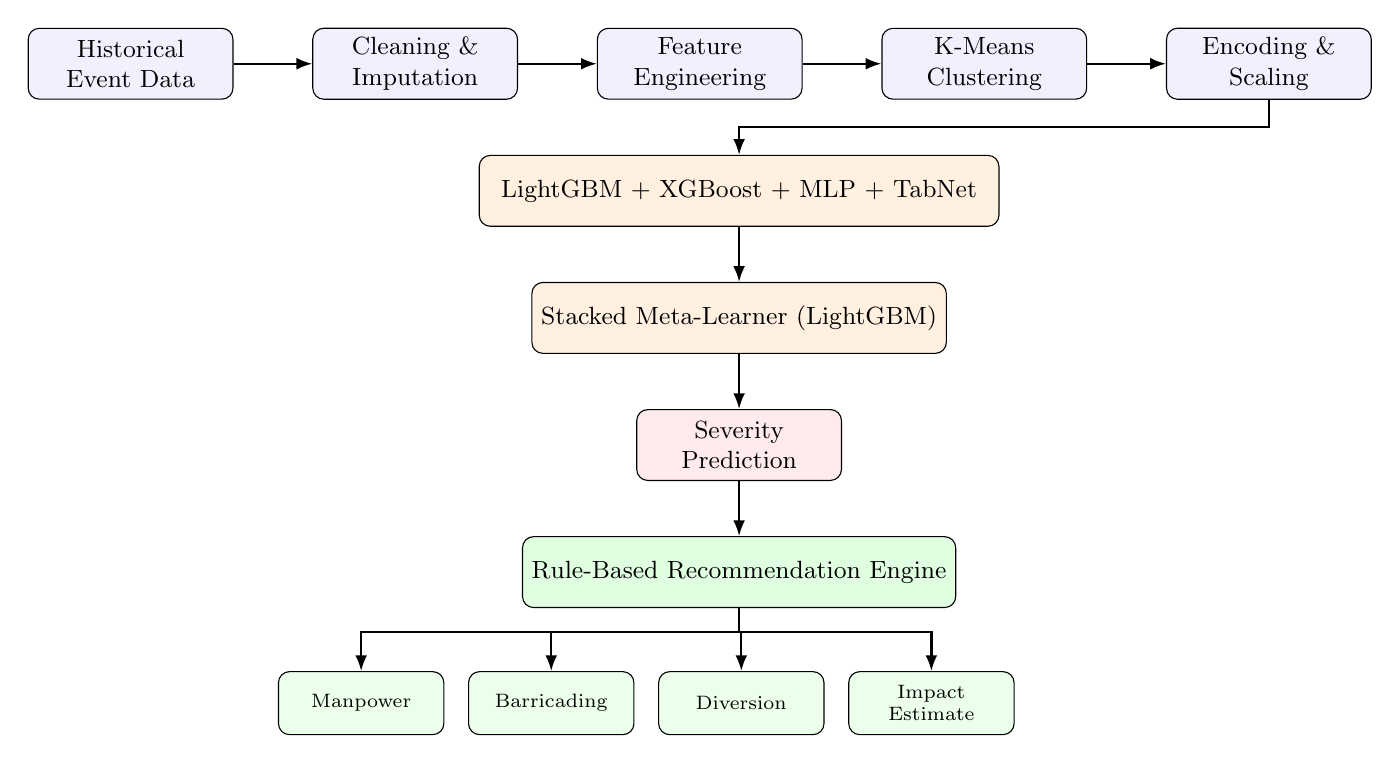
\begin{tikzpicture}[
  node distance = 7mm and 10mm,
  box/.style = {draw, rounded corners, minimum height=0.9cm, minimum width=2.6cm, align=center, font=\small, fill=blue!6},
  stage/.style = {draw, rounded corners, minimum height=0.9cm, minimum width=2.6cm, align=center, font=\small, fill=orange!12},
  outbox/.style = {draw, rounded corners, minimum height=0.8cm, minimum width=2.1cm, align=center, font=\scriptsize, fill=green!8},
  arr/.style = {-{Latex[length=2mm]}, thick}
]
\node[box] (raw) {Historical\\Event Data};
\node[box, right=of raw] (clean) {Cleaning \&\\Imputation};
\node[box, right=of clean] (feat) {Feature\\Engineering};
\node[box, right=of feat] (kmeans) {K-Means\\Clustering};
\node[box, right=of kmeans] (enc) {Encoding \&\\Scaling};

\node[stage, below=of feat, xshift=0.5cm, minimum width=6.6cm] (base) {LightGBM + XGBoost + MLP + TabNet};
\node[stage, below=of base] (meta) {Stacked Meta-Learner (LightGBM)};
\node[box, below=of meta, fill=red!8] (sev) {Severity\\Prediction};
\node[stage, below=of sev, fill=green!12] (rule) {Rule-Based Recommendation Engine};

\node[outbox, below=8mm of rule, xshift=-4.8cm] (o1) {Manpower};
\node[outbox, right=3mm of o1] (o2) {Barricading};
\node[outbox, right=3mm of o2] (o3) {Diversion};
\node[outbox, right=3mm of o3] (o4) {Impact\\Estimate};

\draw[arr] (raw) -- (clean);
\draw[arr] (clean) -- (feat);
\draw[arr] (feat) -- (kmeans);
\draw[arr] (kmeans) -- (enc);
\draw[arr] (enc.south) -- ++(0,-0.35) -| (base.north);
\draw[arr] (base) -- (meta);
\draw[arr] (meta) -- (sev);
\draw[arr] (sev) -- (rule);
\draw[arr] (rule.south) -- ++(0,-0.3) -| (o1.north);
\draw[arr] (rule.south) -- ++(0,-0.3) -| (o2.north);
\draw[arr] (rule.south) -- ++(0,-0.3) -| (o3.north);
\draw[arr] (rule.south) -- ++(0,-0.3) -| (o4.north);
\end{tikzpicture}
\caption{End-to-end system architecture: from raw event data to an operational recommendation.}
\label{fig:architecture}
\end{figure}

\section{Dataset}
\label{sec:dataset}

The dataset is an anonymised export of 8{,}173 historical traffic-event records logged across Bengaluru, with 46 raw attributes covering geographic coordinates, event type and cause, timestamps, corridor and police-jurisdiction identifiers, vehicle information, and resolution/closure details. A column-by-column missingness audit (Figure~\ref{fig:missing}) showed that the 46 raw columns fall into roughly four bands: a handful of columns (\texttt{comment}, \texttt{map\_file}, \texttt{meta\_data}, and several resolution-related fields) are missing in 96--100\% of records and were dropped outright as carrying essentially no signal; a middle band, including \texttt{junction} (69.3\% missing), \texttt{closed\_datetime} (61.6\%), \texttt{zone} (57.9\%), and \texttt{veh\_type} (40.2\%), is missing often enough that dropping it would discard real information, so these columns were retained with an explicit ``unknown'' category or a derived presence flag rather than being imputed as if the value were simply absent; and the remaining columns, including the coordinates, event cause, and priority fields used to build the target, are essentially complete (0\% missing). Pure row identifiers (\texttt{id}, \texttt{client\_id}, \texttt{created\_by\_id}, and similar administrative keys) were dropped regardless of their missingness, since an internal database key carries no geographic or causal signal about severity.

\begin{figure}[!h]
\centering
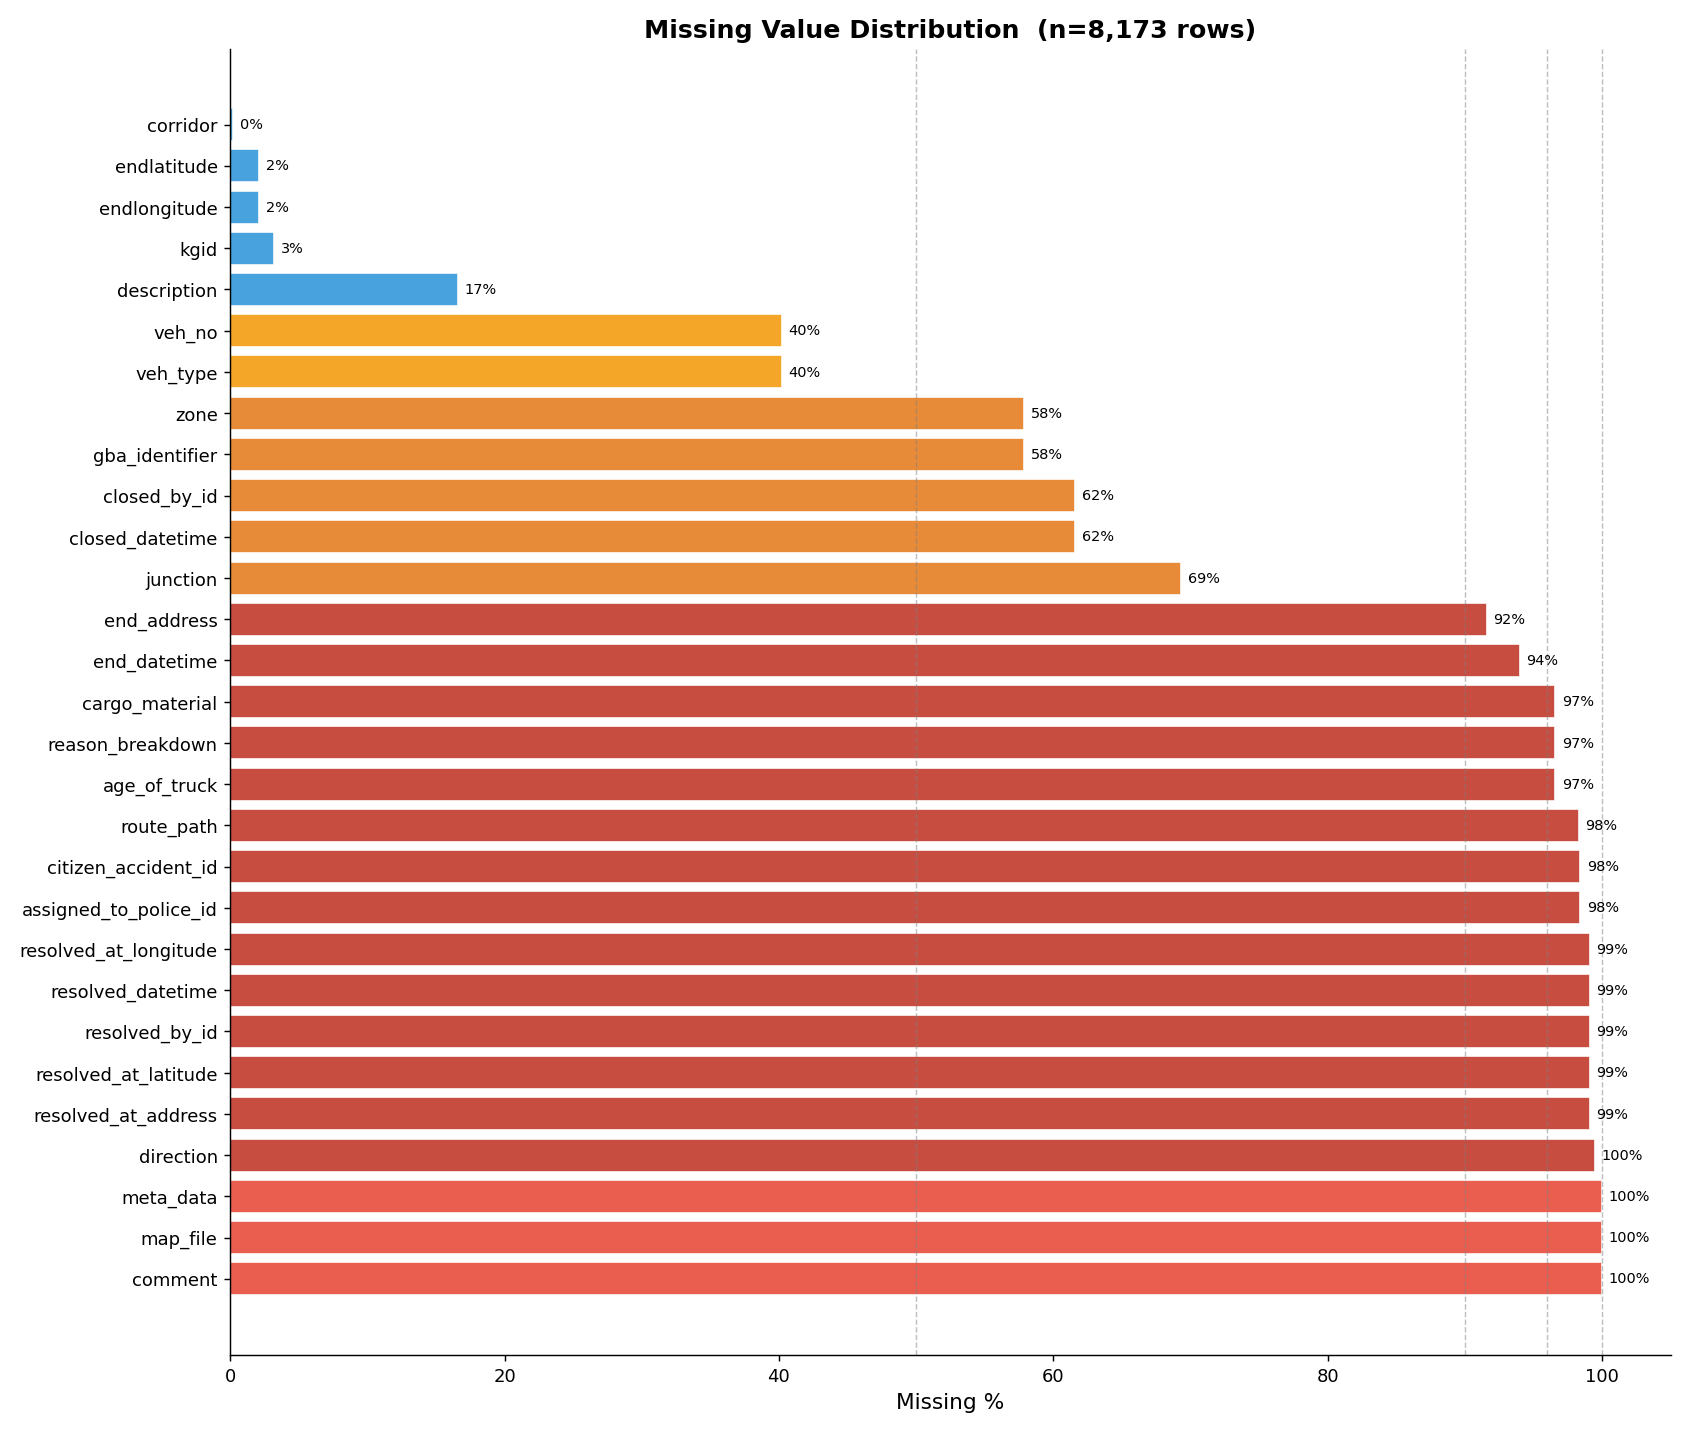
\includegraphics[width=0.85\textwidth]{chapters/5/figs/missing_values.png}
\caption{Missing-value distribution across the 46 raw columns of the event log (n = 8{,}173).}
\label{fig:missing}
\end{figure}

\subsection{Target Variable Construction}
\label{sec:target-construction}

Nowhere in the raw log is there a column that states an event's severity or congestion level directly. The four-class target used throughout this thesis is instead built by combining two fields the control room records independently, for its own operational purposes: the \texttt{priority} tag assigned to the event (High/Low) and whether it \texttt{requires\_road\_closure} (a boolean flag). The four combinations of these two binary fields give a natural four-level ordering, shown in Table~\ref{tab:target-construction}. Both \texttt{priority} and \texttt{requires\_road\_closure} are then removed from the feature set used to train the classifiers -- if they were left in, a model could simply learn the (deterministic) mapping in Table~\ref{tab:target-construction} instead of learning to infer severity from the spatial, temporal, and contextual signals that would actually be available for a genuinely new event.

\begin{table}[!h]
\centering
\caption{Construction of the four-class severity target from two independently recorded fields.}
\label{tab:target-construction}
\begin{tabular}{llcl}
\toprule
Priority & Requires Road Closure & Severity Code & Label \\
\midrule
Low  & No  & 0 & Low \\
Low  & Yes & 1 & Medium \\
High & No  & 2 & High \\
High & Yes & 3 & Critical \\
\bottomrule
\end{tabular}
\end{table}

Table~\ref{tab:class-distribution} and Figure~\ref{fig:target-dist} show the resulting class distribution. The two extreme classes, Low and High, together account for over 91\% of all events, while Medium and Critical make up less than 9\% between them -- Critical events alone are fewer than 300 out of 8{,}173. This confirms, on real data, exactly the imbalance the evaluation methodology in Chapter~\ref{chap:results} is designed around.

\begin{table}[!h]
\centering
\caption{Severity class distribution across all 8{,}173 events.}
\label{tab:class-distribution}
\begin{tabular}{clrr}
\toprule
Code & Label & Count & Percentage \\
\midrule
0 & Low      & 2{,}764 & 33.8\% \\
1 & Medium   &   379   &  4.6\% \\
2 & High     & 4{,}733 & 57.9\% \\
3 & Critical &   297   &  3.6\% \\
\bottomrule
\end{tabular}
\end{table}

\begin{figure}[!h]
\centering
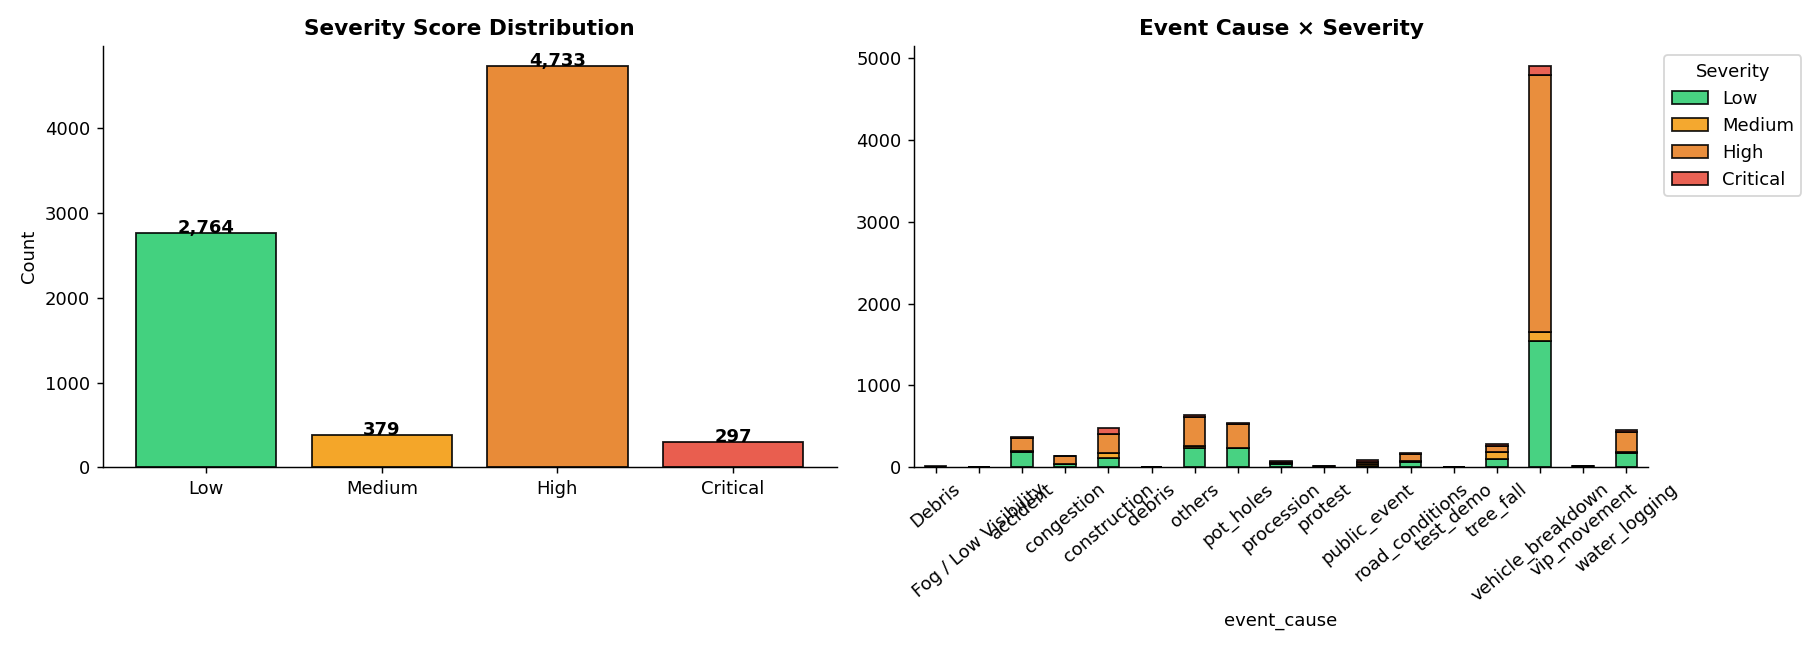
\includegraphics[width=0.95\textwidth]{chapters/5/figs/target_distribution.png}
\caption{Left: severity class counts. Right: how event cause splits across severity levels.}
\label{fig:target-dist}
\end{figure}

\section{Feature Engineering}
\label{sec:feature-engineering}

Thirty features are engineered from the cleaned data and used for modelling, grouped as follows.

\begin{itemize}
\item \textbf{Spatial:} \texttt{latitude}, \texttt{longitude}, \texttt{location\_cluster} (from K-Means, Section~\ref{sec:kmeans}), \texttt{pin\_code} (parsed out of the free-text address field), \texttt{has\_end\_location} (a binary flag, since the raw end-coordinate fields are mostly either genuinely missing or filled with placeholder \texttt{(0, 0)} values that are not real coordinates).
\item \textbf{Temporal:} \texttt{hour}, \texttt{day\_of\_week}, \texttt{month}, \texttt{day}, \texttt{day\_of\_year}, \texttt{is\_weekend}, \texttt{is\_night}, \texttt{is\_morning\_rush} ($7 \le \text{hour} \le 10$), \texttt{is\_evening\_rush} ($17 \le \text{hour} \le 21$), and a coarser \texttt{time\_bucket} category (early morning / morning / afternoon / evening / night / late night).
\item \textbf{Event identity:} \texttt{event\_type}, \texttt{event\_cause}.
\item \textbf{Operational flags:} \texttt{is\_corridor} (whether the event sits on a designated high-density corridor road), \texttt{authenticated\_flag}, \texttt{has\_description}, \texttt{has\_end\_time}, \texttt{has\_been\_closed}.
\item \textbf{Duration / resolution:} \texttt{duration\_mins}, \texttt{resolution\_mins} -- both derived from timestamp differences and clipped to a sensible 0--1440 minute range, with 0 substituted where the underlying timestamp was missing.
\item \textbf{Categorical identifiers:} \texttt{corridor}, \texttt{veh\_type\_simple} (the noisy 40.2\%-null \texttt{veh\_type} field collapsed into five clean buckets -- bus, heavy, private, auto, other/unknown), \texttt{police\_station}, \texttt{zone}, \texttt{junction}, \texttt{status}.
\end{itemize}

After this construction the modelling dataframe has shape $8{,}173 \times 31$ (30 features plus the target), with zero remaining null values. Figure~\ref{fig:correlation} shows each feature's absolute Pearson correlation with the severity target, which is a useful sanity check before training rather than a substitute for the tree-based feature-importance analysis reported later in Section~\ref{sec:feature-importance}.

\begin{figure}[!h]
\centering
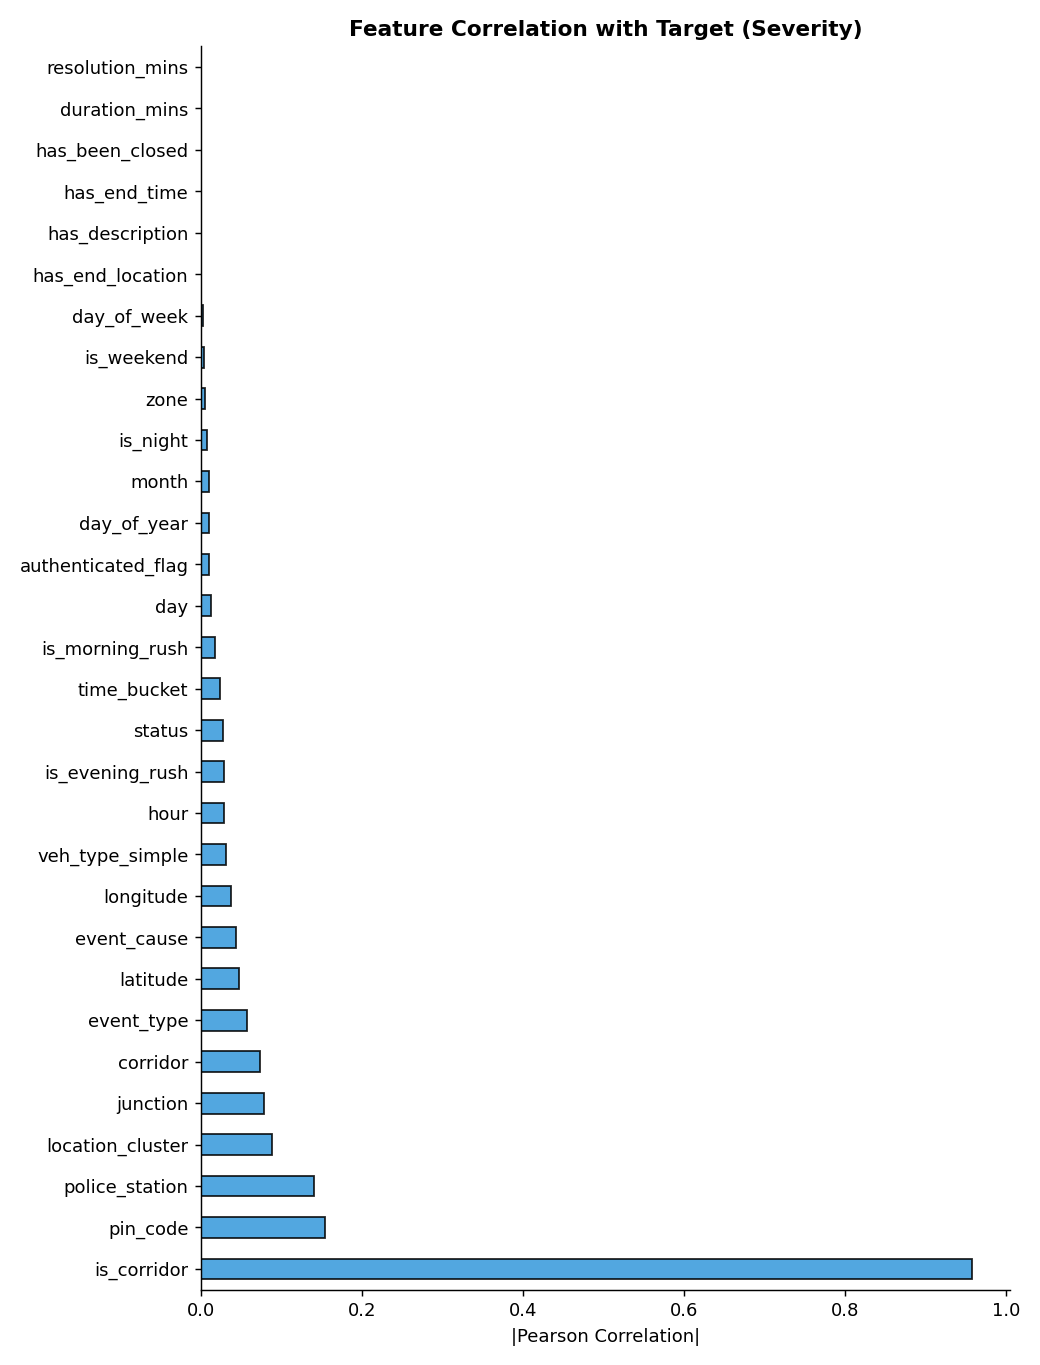
\includegraphics[width=0.7\textwidth]{chapters/5/figs/feature_target_correlation.png}
\caption{Absolute Pearson correlation of each engineered feature with the severity target.}
\label{fig:correlation}
\end{figure}

\subsection{Geographic Clustering with K-Means}
\label{sec:kmeans}

A raw \texttt{(latitude, longitude)} pair on its own gives a classifier very little to generalise from: two events a hundred metres apart have numerically distinct coordinates and are not automatically recognised as belonging to the same neighbourhood. To fix this, the $K$-means clustering algorithm~\cite{macqueen1967methods} is fitted to the event coordinates (using only the 8{,}173 events with valid, non-zero coordinates), with the number of clusters set adaptively as $K = \min(20, \max(5, n/200))$, which for this dataset resolves to $K = 20$. Given $K$ initial centroids, the algorithm alternates between assigning each point to its nearest centroid under Euclidean distance and recomputing each centroid as the mean of its currently assigned points, repeating until the assignment stabilises. The resulting cluster id is stored as \texttt{location\_cluster} and becomes one of the 30 modelling features, letting the downstream classifiers learn region-level severity tendencies -- for instance, a cluster covering a particular high-density corridor experiencing disproportionately more High-severity events -- without needing to memorise raw coordinate values. Figure~\ref{fig:geo-clusters} shows the resulting 20 clusters over Bengaluru.

\begin{figure}[!h]
\centering
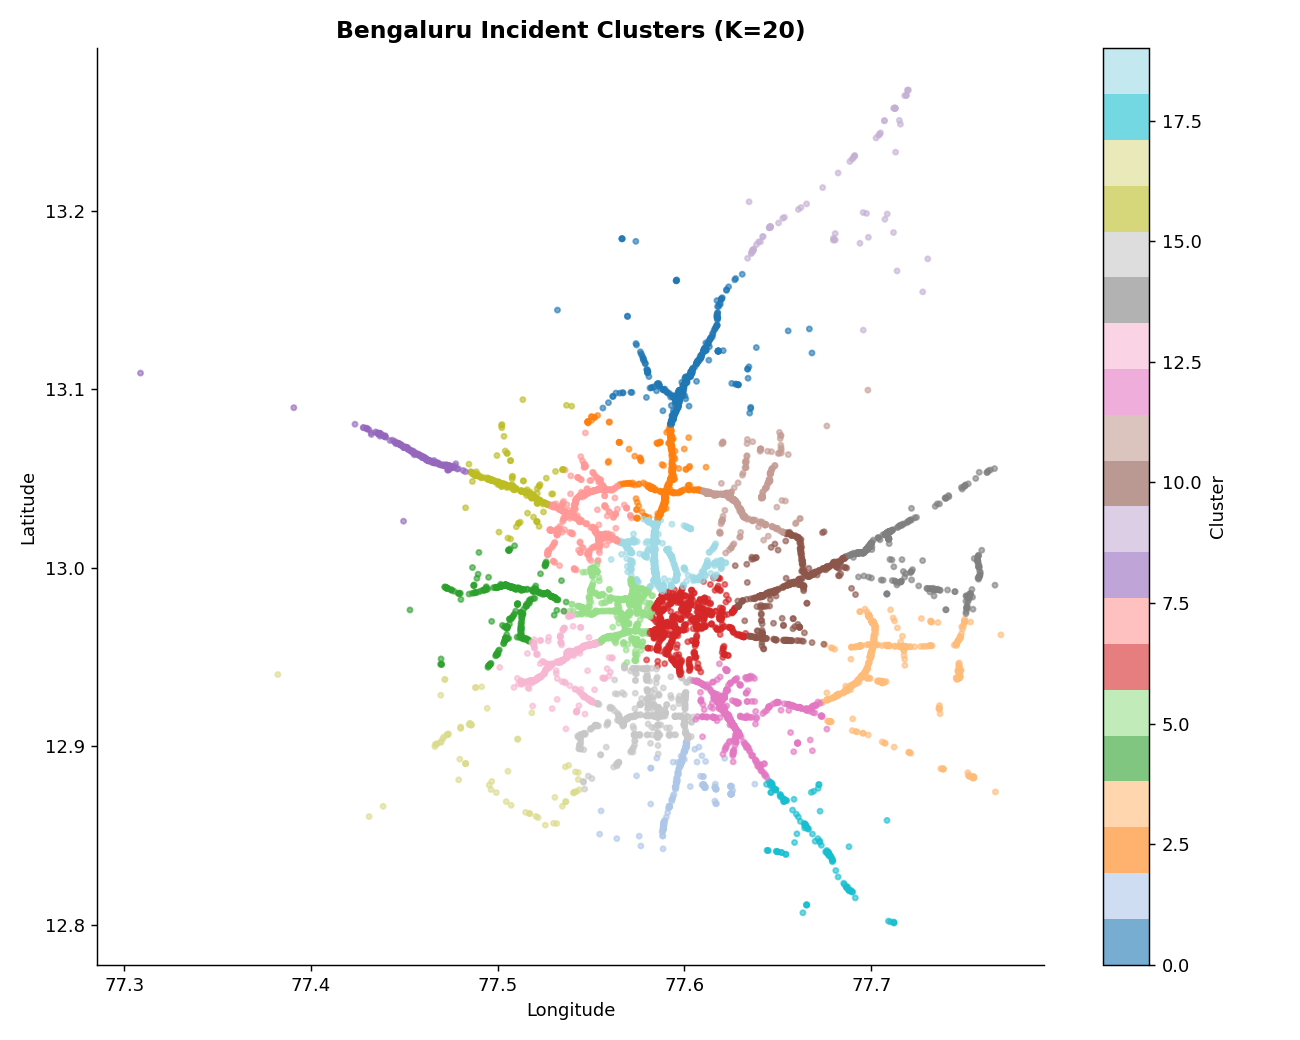
\includegraphics[width=0.65\textwidth]{chapters/5/figs/geo_clusters.png}
\caption{The 20 K-Means geographic clusters fitted over event coordinates across Bengaluru.}
\label{fig:geo-clusters}
\end{figure}

\subsection{Missing-Value Handling and Encoding}

Any numeric column with residual missing values after feature construction is imputed with its column median, which is less sensitive to outliers than the mean. Nine categorical columns -- \texttt{time\_bucket}, \texttt{event\_type}, \texttt{event\_cause}, \texttt{corridor}, \texttt{veh\_type\_simple}, \texttt{police\_station}, \texttt{zone}, \texttt{junction}, \texttt{status} -- are integer-encoded with \texttt{LabelEncoder}, and the fitted encoders are serialized so that the exact same encoding can be reapplied to a new event at inference time (Section~\ref{sec:inference-pipeline}).

\section{Model Training}
\label{sec:base-classifiers}

The 8{,}173 labelled events are split 80/20 into a stratified train/test partition -- 6{,}538 training events and 1{,}635 test events -- preserving the class proportions from Table~\ref{tab:class-distribution} in both splits. Stratification matters here specifically because the Medium and Critical classes are already rare; a plain random split could easily under-represent them further in the test set and make the resulting metrics noisy.

\subsection{Base Classifiers}

Four classifiers are trained independently on the training split.

\begin{itemize}
\item \textbf{LightGBM}~\cite{ke2017lightgbm} -- a histogram-based, leaf-wise gradient-boosted tree ensemble, configured with 1{,}000 estimators, a learning rate of 0.03, 63 leaves, \texttt{feature\_fraction} and \texttt{bagging\_fraction} both at 0.8, balanced class weighting, and L1/L2 regularisation, trained with early stopping (80 rounds) on the held-out test fold.
\item \textbf{XGBoost}~\cite{chen2016xgboost} -- a depth-wise gradient-boosted tree ensemble with 1{,}000 estimators, a learning rate of 0.03, a maximum depth of 6, and row/column sub-sampling of 0.8. XGBoost's scikit-learn interface does not expose a built-in \texttt{class\_weight} option in this configuration, so balanced sample weights are computed explicitly and passed in at fit time; early stopping again uses 80 rounds.
\item \textbf{Multi-Layer Perceptron (MLP)} -- a feed-forward network with hidden layers of size 256, 128, 64, and 32, ReLU activations, and the Adam optimizer~\cite{kingma2015adam}, trained with early stopping (a 15\% validation split, patience of 30 iterations without improvement) to avoid overfitting on a dataset this size. Its inputs are standardised (zero mean, unit variance) before training, since unlike the tree-based models it is sensitive to feature scale.
\item \textbf{TabNet}~\cite{arik2021tabnet} -- an attention-based architecture built specifically for tabular data, configured with a decision/attention embedding width of 32, five sequential decision steps, a sparsity-regularisation coefficient of $10^{-3}$, and the Adam optimizer with a step-decay learning-rate schedule (halving the effective rate roughly every 50 epochs by a factor of 0.9). Training runs for up to 200 epochs with a patience of 30.
\end{itemize}

\subsection{Stacked Ensemble (Meta-Learner)}

Rather than combine the four base models by a simple vote, their class-probability outputs are combined through a stacked ensemble in the sense of Wolpert~\cite{wolpert1992stacked}. To prevent a model's own training data from leaking into the meta-features it later helps predict, out-of-fold (OOF) probabilities are generated with five-fold stratified cross-validation: within each fold, fresh copies of LightGBM, XGBoost, the MLP, and TabNet are trained on the other four folds and used to predict probabilities on the held-out fifth fold. Stacking together the resulting OOF probability vectors -- $4 \times 4 = 16$ dimensions, since each of the four base models outputs a 4-class probability vector -- gives the input to a second LightGBM model, the meta-learner, which learns how much weight to place on each base model's opinion when producing the final severity call.

\section{Rule-Based Resource Recommendation Engine}
\label{sec:recommendation-engine}

A predicted severity code is not, on its own, something a control room can act on -- it still has to be translated into an actual deployment plan. That translation is done by a separate, deterministic rule-based engine, kept intentionally apart from the machine-learning models: the learned models answer ``how severe does this look'', while the rule engine answers ``what do we do about it''. Table~\ref{tab:base-recommendation} gives the base manpower and control-strategy recommendation for each severity level before any contextual adjustment.

\begin{table}[!h]
\centering
\caption{Base severity-to-action mapping used by the recommendation engine.}
\label{tab:base-recommendation}
\small
\begin{tabular}{lp{1.7cm}p{1.4cm}p{4cm}p{4cm}}
\toprule
Severity & Officers (min--max) & Delay est. & Barricading & Diversion \\
\midrule
Low      & 2--4   & 15 min & Cones / indicators only & No diversion needed \\
Medium   & 4--8   & 30 min & Partial barricade (1 lane) + 1 marshal & Advisory alternate route \\
High     & 8--14  & 60 min & Full barricade, both sides, 2 marshal points & Mandatory alternate route + digital signage \\
Critical & 15--25 & 90 min & Full corridor lockdown + marshal chain & Police-escorted diversion + public advisory \\
\bottomrule
\end{tabular}
\end{table}

Two contextual multipliers then adjust this base allocation. If the event is on a designated high-density corridor, the officer range is scaled by $\times 1.4$; if it falls in a peak (rush-hour) window -- 7--10 or 17--21 hours -- the range is scaled by a further $\times 1.25$. Cause-specific rules add extra actions on top of the manpower adjustment: a \texttt{public\_event} of High severity or above triggers a crowd-control-perimeter action and an instruction to coordinate with the event organiser, while an \texttt{accident} of High severity or above triggers an instruction to keep an ambulance lane open and place a trauma centre on standby. For events flagged as pre-announced (planned) rather than sudden, the engine additionally recommends pre-deploying the minimum required officers at least two hours before the event's scheduled start.

\section{Inference Pipeline}
\label{sec:inference-pipeline}

At inference time, a single \texttt{predict\_congestion()} function accepts raw event attributes -- coordinates, event type and cause, start time, corridor and police-station identifiers, vehicle type, expected duration, junction -- and runs the following sequence: (i)~assign the event to its nearest K-Means location cluster; (ii)~construct the same 30 temporal, spatial, and contextual features used in training; (iii)~apply the previously fitted label encoders and standard scaler; (iv)~obtain class probabilities from each of the four base models; (v)~concatenate those probabilities and pass them through the meta-learner to obtain the final severity prediction; and (vi)~pass that prediction, together with event cause, corridor status, and time, to the rule-based recommendation engine to produce the final manpower, barricading, diversion, and delay-estimate output.

\section{Full-Stack Deployment}
\label{sec:fullstack}

The trained pipeline is not left inside the notebook it was developed in -- it is wrapped in a small production-style application so that it can be exercised the way an actual operator would. A Python FastAPI service (the ``ML sidecar'') loads the serialized models, encoders, scaler, and K-Means model once at start-up and exposes the inference pipeline over an internal \texttt{/infer} endpoint. A Go service, built with the Gin framework, sits in front of it as a thin API gateway: it validates incoming requests, forwards them to the sidecar, and exposes the public \texttt{/api/predict}, \texttt{/api/meta}, and \texttt{/api/health} endpoints. A Next.js frontend consumes this API and provides a form for entering an event's details, a Leaflet-based interactive map of Bengaluru, a results view showing the predicted severity, its class-probability breakdown, and the resulting recommendation, and a simple history of past predictions. All three services are containerised and can be brought up together with a single Docker Compose command, which was also the configuration used for deployment (frontend on Vercel, the Go and Python services on Railway).

\clearpage
\thispagestyle{empty}
\newpage

\chapter{Tasks Completed}
\label{chap:tasks}
\noindent \rule{6.6in}{0.01in}
\newpage

The following concrete tasks were completed over the course of this project, roughly in the order they were carried out.

\begin{enumerate}
\item \textbf{Data acquisition and exploratory analysis.} The anonymised 8{,}173-record Bengaluru traffic-event export was loaded and explored: a per-column missingness audit, distribution plots for the key categorical fields (event type, cause, status, priority, corridor, police station), and a temporal breakdown of incident counts by hour of day and day of week.
\item \textbf{Target-variable construction.} A four-class severity target was built from the \texttt{priority} and \texttt{requires\_road\_closure} fields (Section~\ref{sec:target-construction}), and its resulting class distribution was analysed and visualised, confirming the significant class imbalance later central to the evaluation in Chapter~\ref{chap:results}.
\item \textbf{Data cleaning.} Columns with extreme missingness were identified and dropped, datetime fields were parsed, and remaining numeric nulls were median-imputed.
\item \textbf{Feature engineering.} Thirty predictive features were engineered across spatial, temporal, event-identity, operational, and duration/resolution groups, including rush-hour flags and a coarse time-of-day bucket.
\item \textbf{Geographic clustering.} K-Means clustering was applied to event coordinates to generate the \texttt{location\_cluster} feature described in Section~\ref{sec:kmeans}.
\item \textbf{Categorical encoding and scaling.} Nine categorical columns were label-encoded, and a \texttt{StandardScaler} was fitted for the neural-network-based models; both were serialized for reuse at inference time.
\item \textbf{Stratified train/test split.} An 80/20 stratified split (6{,}538 / 1{,}635 events) was performed to preserve class proportions in both partitions.
\item \textbf{Base model training.} LightGBM, XGBoost, an MLP, and TabNet were each trained and evaluated independently on the held-out test set, with a full classification report generated for each.
\item \textbf{Stacked ensemble construction.} A five-fold out-of-fold stacking procedure was implemented and used to train a LightGBM meta-learner on the concatenated base-model probabilities.
\item \textbf{Comparative evaluation.} All five models (the four base models plus the stacked ensemble) were compared on accuracy, macro-F1, and weighted-F1, and per-class precision/recall/F1 was examined in detail, with particular attention to the Critical class.
\item \textbf{Feature-importance analysis.} LightGBM's split-based feature importances were computed and visualised to identify which engineered features most influenced the model's decisions.
\item \textbf{Rule-based recommendation engine.} The severity-to-action mapping described in Section~\ref{sec:recommendation-engine}, including its corridor and peak-hour multipliers and cause-specific special actions, was implemented and demonstrated on four representative event scenarios (Section~\ref{sec:recommendation-demo}).
\item \textbf{End-to-end inference function.} A single \texttt{predict\_congestion()} function integrating feature construction, encoding, base-model prediction, meta-learner combination, and the recommendation engine was implemented (Section~\ref{sec:inference-pipeline}).
\item \textbf{Artifact packaging.} All trained models, the fitted encoders, the scaler, the K-Means model, and the feature-name list were serialized and bundled for downstream reuse.
\item \textbf{Full-stack application.} A Python FastAPI inference sidecar, a Go/Gin API gateway, and a Next.js frontend (with an interactive Leaflet map, a prediction form, a results view, and a prediction history page) were built around the trained pipeline, containerised with Docker Compose, and deployed (frontend on Vercel; the Go and Python services on Railway).
\item \textbf{Report and presentation preparation.} This written thesis report and an accompanying slide presentation summarising the system, methodology, and results were prepared.
\end{enumerate}

\clearpage
\thispagestyle{empty}
\newpage

\chapter{Results and Discussion}
\label{chap:results}
\noindent \rule{6.6in}{0.01in}
\newpage

\section{Overall Model Comparison}

Table~\ref{tab:overall-comparison} and Figure~\ref{fig:model-comparison} summarise how the five models -- the four base classifiers and the stacked ensemble -- perform on the held-out test set of 1{,}635 events. Every model lands in the 89--93\% range on raw accuracy, which at first glance looks like a fairly narrow, unremarkable spread. Macro-F1, which averages performance across all four severity classes \emph{without} weighting by how common each class is, tells a much less flattering story: it ranges from 0.5843 (the MLP) up to 0.6949 (LightGBM), a gap far too large to be explained by the near-identical accuracy figures above it.

\begin{table}[!h]
\centering
\caption{Overall performance on the held-out test set (n = 1{,}635).}
\label{tab:overall-comparison}
\begin{tabular}{lccc}
\toprule
Model & Accuracy & Macro-F1 & Weighted-F1 \\
\midrule
LightGBM         & 0.9223 & \textbf{0.6949} & 0.9148 \\
XGBoost          & 0.9168 & 0.6906 & 0.9114 \\
MLP-NN           & 0.9242 & 0.5843 & 0.8992 \\
TabNet           & \textbf{0.9254} & 0.6027 & 0.9020 \\
Stacked Ensemble & 0.8948 & 0.6639 & 0.8968 \\
\bottomrule
\end{tabular}
\end{table}

\begin{figure}[!h]
\centering
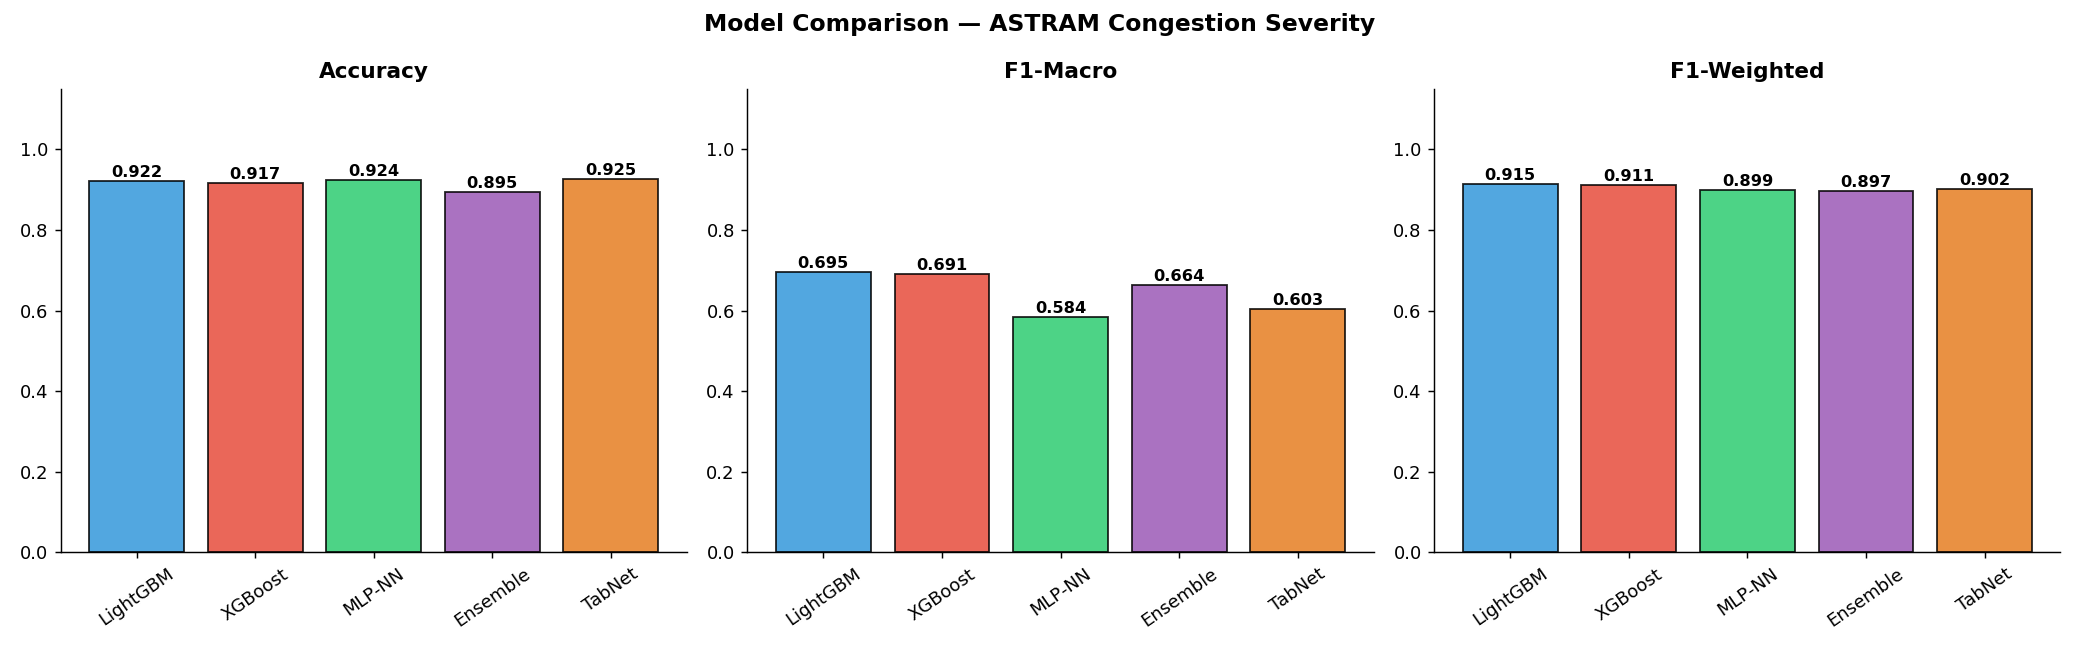
\includegraphics[width=0.95\textwidth]{chapters/7/figs/model_comparison.png}
\caption{Accuracy, macro-F1, and weighted-F1 across all five models.}
\label{fig:model-comparison}
\end{figure}

It is worth flagging the reversal directly: TabNet posts the single highest accuracy of the five models (0.9254), yet it is \emph{not} the best model on macro-F1 -- that title goes to LightGBM, whose accuracy (0.9223) is marginally lower. This is the first sign, examined in depth over the next two sections, that ranking these models by accuracy alone would point a deployment decision in the wrong direction.

\section{Per-Class Performance and the Class-Imbalance Effect}

Table~\ref{tab:critical-class} and Figure~\ref{fig:critical-recall} zoom in on the Critical class specifically, since a missed Critical event is the single costliest mistake this system can make.

\begin{table}[!h]
\centering
\caption{Critical-class precision, recall, and F1-score by model (support = 59).}
\label{tab:critical-class}
\begin{tabular}{lccc}
\toprule
Model & Precision & Recall & F1-score \\
\midrule
LightGBM         & 0.54 & 0.32 & \textbf{0.40} \\
XGBoost          & 0.46 & 0.36 & \textbf{0.40} \\
MLP-NN           & 1.00 & 0.03 & 0.07 \\
TabNet           & 0.75 & 0.10 & 0.18 \\
Stacked Ensemble & 0.28 & 0.34 & 0.31 \\
\bottomrule
\end{tabular}
\end{table}

\begin{figure}[!h]
\centering
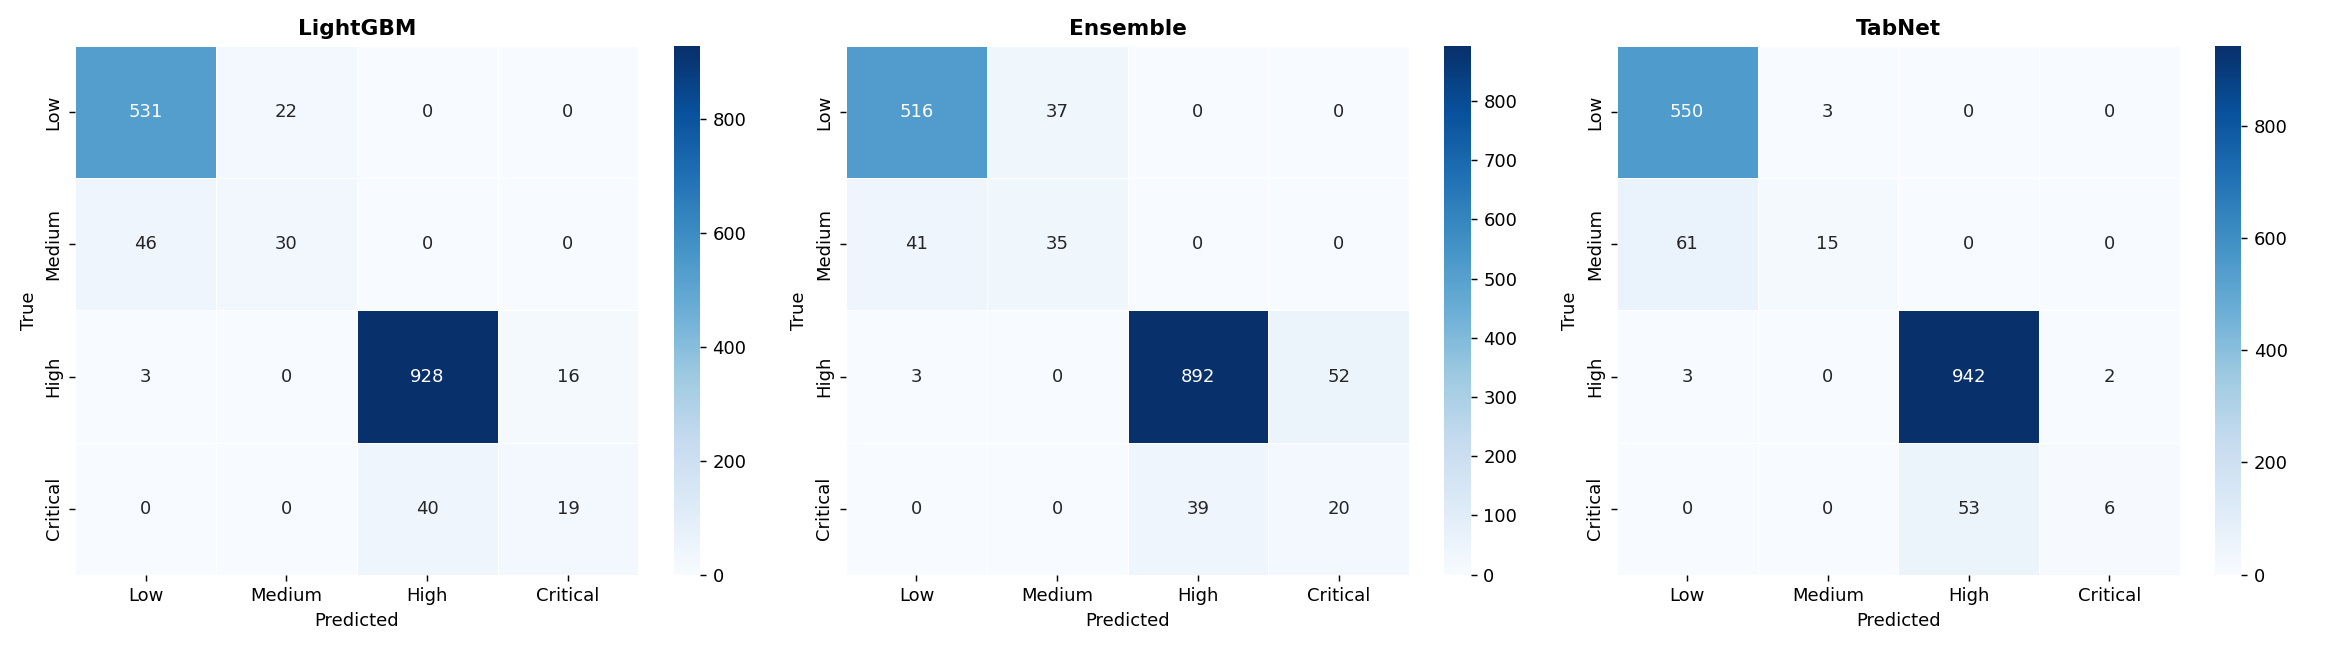
\includegraphics[width=0.75\textwidth]{chapters/7/figs/confusion_matrices.png}
\caption{Confusion matrices for LightGBM, the stacked ensemble, and TabNet on the test set.}
\label{fig:critical-recall}
\end{figure}

The MLP row in Table~\ref{tab:critical-class} is the clearest illustration of the failure mode this thesis is built around: a precision of 1.00 alongside a recall of only 0.03 means that whenever the MLP does predict Critical, it happens to be right every time, but it only makes that prediction for 3\% of the 59 truly Critical events in the test set -- it silently lets the other 97\% through mislabelled as something less urgent. TabNet shows a softer version of the same pattern (75\% precision, 10\% recall). LightGBM and XGBoost, the two models trained with explicit class-balanced sample weighting, behave quite differently: their Critical recall sits at 0.32 and 0.36 respectively, and they end up as the two best-performing models on Critical-class F1 (0.40 each) even though neither of them had the best overall accuracy in Table~\ref{tab:overall-comparison}.

A milder version of the same pattern shows up for the Medium class (Table~\ref{tab:medium-class}): LightGBM and the stacked ensemble share the best Medium-class F1 (0.47), clearly ahead of the MLP (0.36) and TabNet (0.32).

\begin{table}[!h]
\centering
\caption{Medium-class precision, recall, and F1-score by model (support = 76).}
\label{tab:medium-class}
\begin{tabular}{lccc}
\toprule
Model & Precision & Recall & F1-score \\
\midrule
LightGBM         & 0.58 & 0.39 & \textbf{0.47} \\
XGBoost          & 0.56 & 0.39 & 0.46 \\
MLP-NN           & 0.75 & 0.24 & 0.36 \\
TabNet           & 0.83 & 0.20 & 0.32 \\
Stacked Ensemble & 0.49 & \textbf{0.46} & \textbf{0.47} \\
\bottomrule
\end{tabular}
\end{table}

For contrast, all five models handle the two majority classes comfortably -- Low-class F1 sits at 0.93--0.94 and High-class F1 at 0.95--0.97 across the board, regardless of which model is used. The entire spread in Table~\ref{tab:overall-comparison}'s macro-F1 column, in other words, is coming almost entirely from how each model treats the two rarer classes, which is exactly what the accuracy figures alone hide.

\section{Why the Stacked Ensemble Did Not Improve Accuracy}

One result that runs against the usual expectation of stacking is that the ensemble does \emph{not} come out on top of either accuracy or macro-F1 -- it actually posts the lowest raw accuracy of all five models (0.8948), even though its macro-F1 (0.6639) is comfortably ahead of both neural models. Two things plausibly explain this. First, the base models trained inside the five-fold out-of-fold loop were deliberately lighter than their final, fully-tuned counterparts reported in Table~\ref{tab:overall-comparison} -- the in-fold MLP, for instance, uses only two hidden layers (128, 64) rather than the four-layer (256, 128, 64, 32) architecture used for the standalone MLP result -- which likely makes the out-of-fold probability estimates the meta-learner trains on noisier than the probabilities it sees at test time. Second, with only 297 Critical and 379 Medium examples in the whole dataset, five-fold cross-validation leaves each fold with well under 100 examples of either class, which limits how reliably the meta-learner can learn class-specific combination weights for exactly the classes that matter most. Even so, the ensemble still ties for the best Medium-class F1 and posts the second-best Critical recall of all five models, which suggests it is doing what it was built to do -- spreading detection more evenly across classes -- just at some cost to overall accuracy in this particular run.

\section{Why Accuracy Alone Is an Unreliable Metric Here}

Put the two previous sections together and the practical risk becomes concrete rather than abstract: with 91.7\% of the test set being either Low or High severity, a model that leans hard into predicting those two classes can clear 92\% accuracy while missing almost every Critical event it was meant to catch. That is not a hypothetical failure mode -- it is exactly what the MLP does in this experiment, reporting 92.4\% accuracy alongside 3\% Critical recall. That single number pair is the strongest argument in this thesis for reporting macro-F1 and per-class recall throughout, rather than leading with -- or worse, only reporting -- accuracy.

\section{Feature Importance}
\label{sec:feature-importance}

Figure~\ref{fig:feature-importance} shows LightGBM's split-based feature importances, which give a rough sense of which engineered features the strongest base model actually relies on. Spatial and identity-related features -- the geographic cluster from Section~\ref{sec:kmeans}, the corridor and police-station identifiers, and the event cause -- sit near the top, alongside the duration and resolution fields, which is consistent with severity being driven jointly by \emph{where} an event happens and \emph{what kind} of event it is, rather than by any single dominant feature.

\begin{figure}[!h]
\centering
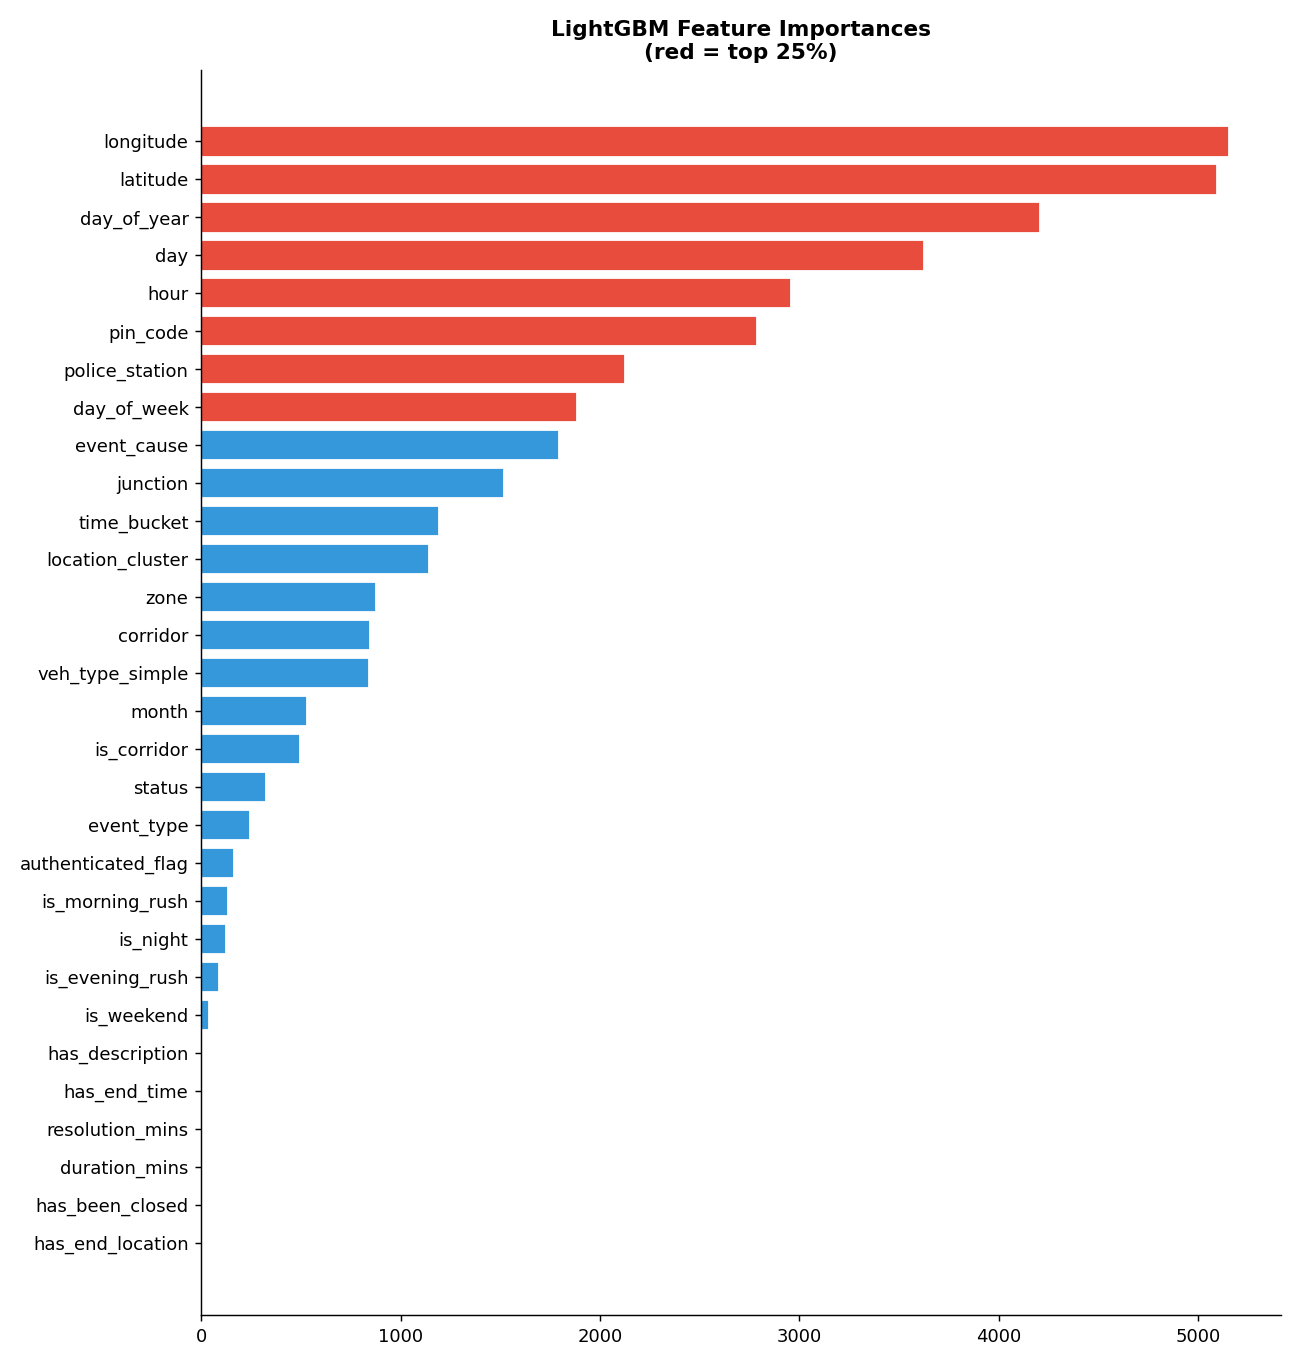
\includegraphics[width=0.7\textwidth]{chapters/7/figs/lgbm_feature_importance.png}
\caption{LightGBM feature importances (split count), red bars mark the top quartile.}
\label{fig:feature-importance}
\end{figure}

\section{Recommendation Engine: Demonstration}
\label{sec:recommendation-demo}

Table~\ref{tab:recommendation-demo} shows the rule-based recommendation engine's output for four representative scenarios, one at each severity level, illustrating how the base severity-to-action mapping in Table~\ref{tab:base-recommendation} is adjusted by corridor and peak-hour context.

\begin{table}[!h]
\centering
\caption{Recommendation engine output for four demonstration scenarios.}
\label{tab:recommendation-demo}
\small
\begin{tabular}{p{3.3cm}p{1.6cm}p{2.6cm}p{2.6cm}p{2.9cm}}
\toprule
Scenario & Manpower & Barricading & Diversion & Special action \\
\midrule
Low, vehicle breakdown, non-corridor, 14:00 & 2--4 officers & Cones only & None & -- \\
\addlinespace
Medium, water-logging, non-corridor, 09:00 (peak) & 5--10 officers & Partial barricade & Advisory route & Peak-hour +25\% flagged \\
\addlinespace
High, public event, corridor, 18:00 (peak), planned & 13--23 officers & Full barricade & Mandatory diversion & Crowd-control perimeter; pre-deploy $\geq$2h \\
\addlinespace
Critical, public event, corridor, 19:00 (peak), planned & 26--43 officers & Full corridor lockdown & Police-escorted diversion & Crowd-control perimeter; pre-deploy $\geq$2h \\
\bottomrule
\end{tabular}
\end{table}

The High- and Critical-severity ranges in Table~\ref{tab:recommendation-demo} (13--23 and 26--43 officers) are exactly what falls out of applying both the corridor multiplier ($\times 1.4$) and the peak-hour multiplier ($\times 1.25$) to the base ranges in Table~\ref{tab:base-recommendation}, which confirms the contextual-adjustment logic is behaving as designed rather than by coincidence.

\section{Summary of Findings}

Three conclusions fall out of the results above. First, every model tested is capable of predicting overall severity with high accuracy, which says the engineered feature set genuinely carries a strong signal -- this is not a case where the modelling choices are struggling against unusable inputs. Second, that shared high accuracy conceals a large, consistent gap in how well each model detects the minority classes, and the two class-weighted tree models (LightGBM and XGBoost) are noticeably more dependable on the operationally important Medium and Critical classes than either neural model trained without explicit class weighting here. Third, the rule-based recommendation layer, despite being intentionally simple and entirely deterministic, does successfully turn a bare severity label into a differentiated, context-sensitive operational plan, which supports the two-stage ``predict, then decide'' design chosen for this system back in Section~\ref{sec:recommendation-engine}.

\section{Limitations}

A few limitations are worth stating plainly. The severity label itself is a constructed proxy, built from two administrative fields rather than an independently annotated ground truth, so what the models are really learning to reproduce is this particular labelling policy -- not necessarily an external, universally agreed notion of ``true'' severity. The evaluation rests on a single stratified train/test split rather than repeated cross-validation, so the reported numbers carry some sampling variance, and that variance is largest precisely for the rare Medium and Critical classes where each percentage point corresponds to only a handful of events. Finally, the system has been tested only offline against historical records; it has not been run in a live control room, and its recommendations have not been checked against what a human operator would actually have decided for the same events.

\section{Conclusion and Future Scope}
\label{sec:future-scope}

This thesis set out to build, end to end, a system that predicts event-driven traffic-congestion severity and turns that prediction into an actionable resource recommendation, using a real, anonymised log of 8{,}173 Bengaluru traffic events. Four classifiers with different structural biases were trained and combined through a stacked ensemble, and every one of them was evaluated with explicit, front-loaded attention to class imbalance rather than accuracy alone. The headline result is that overall accuracy is a poor proxy for real usefulness here: only the class-weighted tree models, and to a lesser extent the stacked ensemble, achieve acceptable recall on the rare but safety-critical Critical class, which has direct implications for how a system like this would need to be tuned -- and which model would need to be chosen -- before any real deployment.

A few concrete directions follow naturally from what the results exposed.

\begin{itemize}
\item \textbf{Explicit class-imbalance handling.} Systematically compare class-weighting, SMOTE-based oversampling~\cite{chawla2002smote}, and decision-threshold adjustment specifically for the Medium and Critical classes, and measure their effect on macro-F1 and Critical recall rather than assuming any one of them is sufficient on its own.
\item \textbf{Ablation studies.} Isolate the individual contribution of the K-Means location-cluster feature and of the stacking step itself by comparing performance with and without each component, holding everything else fixed.
\item \textbf{Richer real-time context.} Bring in live weather data, a real-time traffic-flow feed, and road-network graph structure to complement the currently static, event-record-based feature set.
\item \textbf{Independent severity ground truth.} Where feasible, replace or augment the current priority/closure-derived label with severity judgements from an independent source -- for instance, retrospective control-room review -- to check whether the models are learning genuine severity signal or only the administrative labelling policy behind Table~\ref{tab:target-construction}.
\item \textbf{Field pilot.} Run the inference pipeline alongside real human traffic-control decision-making in a controlled pilot, comparing recommended and actual resource allocations, and use that comparison to refine the rule-based engine iteratively.
\end{itemize}

\clearpage
\thispagestyle{empty}
\newpage

\addtocounter{page}{-1}
\appendix
%%%..........................................................................................................................................
%\fancychapter{Appendix}\label{Sunil_Appendix}
%\chapter{Appendix}\label{Sunil_Appendix}
%  \include{Chapters/Appendix/Appendix}
%\clearpage
%%..........................................................................................................................................
%\fancychapter{Cepstral Analysis}
%\label{app:lpc}
%\include{chapters/Appendix/CFA}
%\clearpage
%%..........................................................................................................................................
%\fancychapter{Linear Prediction Coefficients Computation}
%\label{app:sine}
%\include{chapters/Appendix/Appendix_lpc_V2}
%\clearpage
%%..........................................................................................................................................
%\fancychapter{Composite Objective Quality Measures}
%\label{app:cqm}
%\include{Chapters/Appendix/Appendix_cqm_V1}
%\clearpage
%%..........................................................................................................................................
%\fancychapter{MFCC Feature Extraction}
%\label{app:mfcc}
%\include{Chapters/Appendix/Appendix_mfcc_V1}
%\clearpage
%%..........................................................................................................................................
%\fancychapter{Gaussian Mixture Models}
%\label{app:gmm}
%\include{Chapters/Appendix/Appendix_gmm_V1}
%\clearpage
%..........................................................................................................................................
%\doublespacing
%\normalsize
%\pdfbookmark{Publications}{Publications}
%\fancyhead[LE]{\bfseries\small{List of Publications}}
%\fancyhead[RO]{\bfseries\small{List of Publications}}
%\pdfbookmark[1]{List of Publications}{los}
%\addstarredchapter{List of Publications}
%\include{FrontPages/publ}
%\clearpage

%% LIST OF SYMBOLS
%\fancyhead[LE]{\bfseries\small{List of Symbols}}
%\fancyhead[RO]{\bfseries\small{List of Symbols}}
%\pdfbookmark[1]{List of Symbols}{los}
%\addstarredchapter{List of Symbols}
%\include{FrontPages/Symbols}
%\clearpage
%******************************************************************************************************************************************************************

%**************************************************BIBLIOGRAPHY********************************************************
\fancyhead[LE]{\bfseries\small{Bibliography}}
\fancyhead[RO]{\bfseries\small{Bibliography}}
\pdfbookmark[1]{Bibliography}{los}
\addstarredchapter{Bibliography}   % PKM 05/07/08 (For more options refer minitoc.pdf on page 36)
\baselineskip 14pt   %12, 18 and 24
\small
\bibliographystyle{IEEEtran}
\bibliography{chapters/references/MyBibliography_database_Maninder}
%\clearpage
%**************************************************PUBLICATIONS****************************************************************************************************************



\end{document}
